\documentclass[9pt,a4paper]{article}

\usepackage[margin=1in]{geometry}
\usepackage{amsmath,amssymb,amsthm}
\usepackage{xcolor}
\usepackage{array}
\usepackage{tabularx}
\usepackage{hyperref}
\usepackage{microtype}
\usepackage{float}
\usepackage{booktabs}
\usepackage{graphicx}
\usepackage{tikz}
\usetikzlibrary{arrows,positioning,fit,backgrounds,shapes.geometric}
\usepackage[ruled,vlined,linesnumbered]{algorithm2e}

\usepackage{fontspec}
\usepackage{unicode-math}

\setmainfont{DejaVu Serif}
\setsansfont{DejaVu Sans}
\setmonofont{DejaVu Sans Mono}[Scale=MatchLowercase]
\setmathfont{STIX Two Math}

\usepackage{agda}
\usepackage{agda-spec}

\renewcommand{\AgdaFontStyle}[1]{{\small\sffamily #1}}
\renewcommand{\AgdaKeywordFontStyle}[1]{{\small\sffamily\bfseries #1}}
\renewcommand{\AgdaBoundFontStyle}[1]{{\small\sffamily\itshape #1}}
\renewcommand{\AgdaStringFontStyle}[1]{{\small\ttfamily #1}}
\renewcommand{\AgdaCommentFontStyle}[1]{{\small\ttfamily #1}}

\definecolor{AgdaComment}      {HTML}{616E88}
\definecolor{AgdaPragma}       {HTML}{616E88}
\definecolor{AgdaKeyword}      {HTML}{5E81AC}
\definecolor{AgdaString}       {HTML}{A3BE8C}
\definecolor{AgdaNumber}       {HTML}{B48EAD}
\definecolor{AgdaSymbol}       {HTML}{4C566A}

\definecolor{AgdaBound}                 {HTML}{2E3440}
\definecolor{AgdaGeneralizable}         {HTML}{5E81AC}
\definecolor{AgdaInductiveConstructor}  {HTML}{8FBCBB}
\definecolor{AgdaCoinductiveConstructor}{HTML}{88C0D0}
\definecolor{AgdaDatatype}              {HTML}{81A1C1}
\definecolor{AgdaField}                 {HTML}{B48EAD}
\definecolor{AgdaFunction}              {HTML}{5E81AC}
\definecolor{AgdaMacro}                 {HTML}{A3BE8C}
\definecolor{AgdaModule}                {HTML}{E0BA62}
\definecolor{AgdaPostulate}             {HTML}{BF616A}
\definecolor{AgdaPrimitive}             {HTML}{81A1C1}
\definecolor{AgdaRecord}                {HTML}{81A1C1}
\definecolor{AgdaArgument}              {HTML}{4C566A}

\urlstyle{tt}
\newcommand{\fpath}[1]{\nolinkurl{#1}}

\theoremstyle{plain}
\newtheorem{theorem}{Theorem}
\newtheorem{lemma}[theorem]{Lemma}
\newtheorem{corollary}[theorem]{Corollary}
\theoremstyle{definition}
\newtheorem{definition}{Definition}
\theoremstyle{remark}
\newtheorem{remark}{Remark}

\title{\textbf{Compact Policy Synthesis via Coinductive Rankings} \\
Boolean Predicates for Continuous Control---Methods and Experiments}

\author{Ricardo Corral-Corral}
\date{April 2026}

\begin{document}

\maketitle

\begin{abstract}
Coinductive Symmetric Homomorphism Reinforcement Learning
(CSHRL)~\cite{CSHRL2026} encodes optimality as a structural
property of \emph{rankings}---total preorders over the action
space---rather than as the maximization of a scalar return.
The formal synthesis theory (CEGIS, propagation, sample
bounds) is developed in a companion paper~\cite{CSHRLSynthesis2026},
where the entire pipeline lives inside the Agda proof assistant.
That pipeline is limited to environments Agda can model natively.

This paper documents a \textbf{predicate synthesis} approach
that scales CSHRL-inspired ideas beyond what pure Agda can
handle.  The core question is: \emph{can the decision structure
of standard RL benchmarks be captured by a handful of Boolean
predicates?}  We explore this through heuristic search
strategies---CEGAR-style refinement, coordinate descent,
partition enumeration, binary-weighted decomposition---that
discover predicates by evaluating candidates against
simulated episodes.  The search is not formally verified;
it relies on rollout aggregates and episode-reward scoring.
What it preserves is the \emph{output format}: compact,
interpretable Boolean-predicate policies.

We explore four synthesis strategies---flat-partition CEGAR,
coordinate descent with episode-reward ranking, partition-based
exhaustive search, and binary-weighted decomposition for
continuous actions---across \textbf{twelve environments}:
Pendulum, LunarLander, CartPole, MountainCar, Acrobot, Pong,
Breakout, BipedalWalker, Swimmer (MuJoCo), CliffWalking,
Slippery CliffWalking, and FrozenLake 8$\times$8 Slippery.
All are solved with \textbf{1--12 Boolean predicates} and
zero neural network parameters.  The headline result is compactness: the entire
decision structure of each benchmark fits in a handful of
human-readable inequalities over physics variables.

The LunarLander controller, for example, is three predicates:
\begin{center}
\texttt{if $5\omega^2 + \theta < 0 \wedge \theta < 2x$:
left $>$ noop $>$ right $>$ main} \\
\texttt{if $x < 4\theta \wedge v_x < 5\omega$:
right $>$ noop $>$ left $>$ main} \\
\texttt{if $v_y < {-}0.1 \wedge 2v_y + y < 0$:
main $>$ left $>$ noop $>$ right} \\
\texttt{else: noop $>$ left $>$ right $>$ main}
\end{center}
\end{abstract}

%% ================================================================
\section{Introduction}
%% ================================================================

CSHRL~\cite{CSHRL2026} provides a coinductive framework for
reinforcement learning based on \emph{rankings}---total preorders
over the action space at each state---rather than value functions.
A ranking is a \emph{Coinductive Homomorphism} (CoindHomo) when it
is self-consistent under the agent's own dynamics: if the ranking
says action~$a$ is at least as good as action~$b$ at state~$s$,
the value stream from taking~$a$ dominates the stream from~$b$,
coinductively, along the infinite trajectory.  The formal synthesis
theory---PredProg DSL, CEGIS, propagation, sample complexity
bounds---is developed in the companion
paper~\cite{CSHRLSynthesis2026}, where everything lives inside
Agda: observations drive a version-space search, and the
type-checker certifies the result.

That purely formal pipeline works for environments Agda can model
natively---CartPole, MountainCar, FrozenLake---but it cannot
scale to environments with complex physics or high-dimensional
continuous state spaces.  This paper documents the
\textbf{predicate synthesis} approach that bridges that gap:
heuristic search strategies discover Boolean predicates by
evaluating candidates against simulated episodes, while
the formal CSHRL theory provides the \emph{conceptual} backbone
---rankings, coinductive consistency, predicate programs.
The implementation (Synthex, in Elixir) uses Gymnasium as the
environment interface, but the ideas are independent of any
particular simulator.

\subsection{What Synthex Is---and What It Is Not}

Synthex is \textbf{CSHRL-inspired}, not a faithful implementation
of the formal synthesis pipeline.  Several design choices trade
formal guarantees for empirical scalability:

\begin{itemize}
\item \textbf{Ranking by rollout aggregates.}  Instead of
      computing coinductive stream comparisons, Synthex scores
      actions by aggregate episode reward or terminal-state
      penalty over finite rollout batches.  These are noisy
      proxies, not the pointwise stream dominance that CoindHomo
      demands.

\item \textbf{Heuristic search.}  Predicates are discovered by
      coordinate descent, CEGAR-style counterexample splitting,
      or partition enumeration.  None of these search strategies
      guarantees finding the optimal ranking---they find
      \emph{good} rankings under the scoring heuristic.

\item \textbf{Partial verification.}  Discovered predicates
      \emph{can} be fed back to Agda for CoindHomo certification,
      but this requires an Agda-side dynamics model.  Where
      the Agda model diverges from the real environment
      (e.g., Euler integration vs.\ Box2D physics), the
      certificate does not transfer.  In practice, only a
      subset of predicates achieve \texttt{refl} proofs.

\item \textbf{Full-ranking determination.}  The formal theory
      requires a complete action permutation per state region.
      Synthex approximates this by independently scoring each
      action via episode reward---a heuristic that produces
      plausible rankings but is not guaranteed to recover the
      true coinductive ordering.
\end{itemize}

The value of the Synthex approach is not formal verification---it
is that the output remains a \textbf{compact, interpretable
Boolean-predicate policy}.  Every environment in this paper is
solved with 1--12 predicates and zero neural network parameters.
The policies are human-readable, portable to any language, and
their decision structure is transparent by inspection.  This
compactness is itself a scientific finding about the environments:
standard RL benchmarks have fundamentally low-dimensional decision
structure, and deep RL's parameter overhead is spent on
representation, not on decision complexity.

\subsection{Rankings and Coinductive Consistency}

A ranking defines a total preorder~$\le$ over actions.  At an
absorbing fixed point (e.g., equilibrium), all actions lead to
equivalent successor states, so $a \le b$ and $b \le a$ for every
pair.  Every permutation is a valid linearization---the optimal
policy at equilibrium is genuinely non-unique.  This falls out
transparently from using~$\le$ rather than~$<$.

The \textbf{terminal-state ranking criterion} makes the coinductive
structure computationally explicit: action~$a$ ranks above~$b$
when the trajectory from~$a$ arrives at a superior state at the
lookahead horizon.  The terminal state is the continuation point
for the next coinductive step.  One-step comparisons are
short-sighted: the immediate successor from~$a$ may have worse
penalty than from~$b$, yet $a$ is the superior action because it
bridges to a far-future state that dominates $b$'s terminal state.

\subsection{Synthesis Strategies: A Zoo of Approaches}

The synthesis produces a \textbf{flat partition} of the state space:
an ordered list of (predicate, full-ranking) pairs with a default.
Each state falls into the first matching region, which assigns a
complete action permutation.  Four search strategies handle
different problem structures:

\begin{enumerate}
\item \textbf{Flat-partition CEGAR} (\S\ref{sec:flat-cegar}):
      a terminal-state oracle ranks actions, and a CEGAR loop
      splits regions to resolve disagreements.  Suitable for
      stabilization tasks with a geometric penalty (Pendulum).

\item \textbf{Coordinate descent} (\S\ref{sec:coorddescent}):
      optimizes one predicate position at a time via episode
      reward, then lifts the top-action chain to a full ranking.
      Efficient when predicates show independent improvement
      (LunarLander, CartPole, MountainCar, Acrobot, Pong,
      Breakout).

\item \textbf{Partition-based search} (\S\ref{sec:partition}):
      jointly enumerates predicate sets and action assignments.
      Necessary when predicates are correlated and no single
      predicate improves reward in isolation
      (CliffWalking, FrozenLake).

\item \textbf{Binary-weighted decomposition} (\S\ref{sec:bipedal}):
      maps continuous action dimensions to independent binary
      sub-actions, each synthesized as an independent 2-action
      problem.  Extends the framework to continuous action
      spaces (BipedalWalker, Swimmer).
\end{enumerate}

All four produce the same kind of output---Boolean predicates over
continuous state features---but they differ in search strategy,
ranking criterion, and the environments they suit.  No single
method dominates; the choice is environment-dependent.  This is an
evolving research program: we present the methods as a landscape
of approaches, not as a settled pipeline.

\begin{figure}[t]
\centering
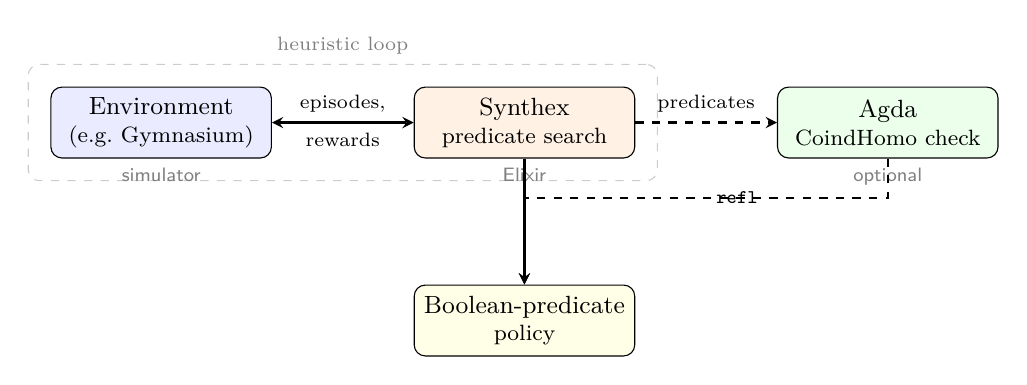
\begin{tikzpicture}[
  node distance=1.2cm and 1.8cm,
  box/.style={draw, rounded corners, minimum width=2.8cm,
              minimum height=0.9cm, align=center, font=\small},
  lang/.style={font=\scriptsize\sffamily, text=gray},
  arr/.style={-stealth, thick},
  darr/.style={stealth-stealth, thick},
]
\node[box, fill=blue!8] (gym) {Environment\\[-1pt]\footnotesize (e.g.\ Gymnasium)};
\node[lang, below=0pt of gym] {simulator};

\node[box, fill=orange!10, right=of gym] (synthex) {Synthex\\[-1pt]\footnotesize predicate search};
\node[lang, below=0pt of synthex] {Elixir};

\node[box, fill=green!8, right=of synthex] (agda) {Agda\\[-1pt]\footnotesize CoindHomo check};
\node[lang, below=0pt of agda] {optional};

\node[box, fill=yellow!10, below=1.6cm of synthex] (policy)
     {Boolean-predicate\\[-1pt]\footnotesize policy};

\draw[darr] (gym) -- node[above, font=\scriptsize]
     {episodes,} node[below, font=\scriptsize] {rewards} (synthex);
\draw[arr, dashed] (synthex) -- node[above, font=\scriptsize]
     {predicates} (agda);
\draw[arr] (synthex) -- (policy);
\draw[arr, dashed] (agda.south) -- ++(0,-0.5)
     -| node[near start, right, font=\scriptsize] {\texttt{refl}} (policy);

\begin{scope}[on background layer]
  \node[draw=gray!40, dashed, rounded corners, inner sep=8pt,
        fit=(gym)(synthex), label={[font=\scriptsize,
        text=gray]above:heuristic loop}] {};
\end{scope}
\end{tikzpicture}
\caption{Synthesis architecture.  The core loop (left, dashed box) is
heuristic: the search engine proposes predicates, the environment
evaluates them via episode rollouts, and the best candidates survive.
Agda verification is optional and requires a dynamics model that may
diverge from the simulator.  The output in all cases is a compact
Boolean-predicate policy.}
\label{fig:pipeline}
\end{figure}

\subsection{Methods Landscape}

Table~\ref{tab:methods} summarizes the four synthesis strategies,
the environments where each has been applied, and the key
trade-offs.  The ranking criterion column indicates how actions
are scored: by \emph{terminal-state penalty} (comparing the state
reached at the end of a fixed lookahead), by \emph{episode reward}
(running a complete episode and using the cumulative return), or
by \emph{per-bit episode reward} (scoring each binary sub-action
independently).

\begin{table}[t]
\centering
\small
\begin{tabular}{@{}p{3.2cm}p{2.5cm}p{2.8cm}p{4.5cm}@{}}
\toprule
\textbf{Strategy} & \textbf{Ranking criterion} & \textbf{Environments} &
  \textbf{Trade-offs} \\
\midrule
Flat-partition CEGAR
  (\S\ref{sec:flat-cegar})
  & Terminal-state penalty
  & Pendulum
  & Requires a geometric penalty function; ranking quality depends
    on the follow-up policy (chicken-and-egg) \\
\addlinespace
Coordinate descent
  (\S\ref{sec:coorddescent})
  & Episode reward
  & LunarLander, CartPole, MountainCar, Acrobot, Pong, Breakout
  & Efficient when predicates improve reward independently;
    full ranking is heuristically determined post-hoc, not
    guaranteed to match the true coinductive ordering \\
\addlinespace
Partition-based search
  (\S\ref{sec:partition})
  & Episode reward (joint)
  & CliffWalking, Slippery CliffWalking, FrozenLake
  & Handles correlated predicates; exponential in partition
    size, feasible only for small action/feature counts \\
\addlinespace
Binary-weighted decomposition
  (\S\ref{sec:bipedal})
  & Per-bit episode reward
  & BipedalWalker, Swimmer
  & Scales linearly in action dimensions; each bit is an
    independent 2-action problem; resolution limited by
    bit count \\
\bottomrule
\end{tabular}
\caption{Synthesis strategies and their characteristics.  No single
method dominates; the choice depends on the environment's structure.}
\label{tab:methods}
\end{table}

%% ================================================================
\section{The Predicate DSL}
%% ================================================================

The predicate DSL is the shared language between synthesis and
verification. A \texttt{PredProg} is a Boolean combination of
feature tests over a generic carrier type.

\begin{spec}
{-# OPTIONS --safe --guardedness #-}
module HybridSynthesis where

open import Data.Bool
  using (Bool; true; false; if_then_else_; _∧_; _∨_; not)
open import Data.List using (List; []; _∷_)
open import Data.Nat  using (ℕ; zero; suc; _+_; _≤ᵇ_; _∸_)
open import Data.Product using (_×_; _,_)
open import Relation.Binary.PropositionalEquality using (_≡_; refl)

module PredDSL
  (State   : Set)
  (Feature : Set)
  (eval-feature : Feature → State → Bool)
  where

  data PredProg : Set where
    feat   : Feature → PredProg
    _∧p_   : PredProg → PredProg → PredProg
    _∨p_   : PredProg → PredProg → PredProg
    ¬p_    : PredProg → PredProg
    truep  : PredProg
    falsep : PredProg

  infixr 6 _∧p_
  infixr 5 _∨p_

  eval : PredProg → State → Bool
  eval (feat f)  s = eval-feature f s
  eval (p ∧p q)  s = eval p s ∧ eval q s
  eval (p ∨p q)  s = eval p s ∨ eval q s
  eval (¬p p)    s = not (eval p s)
  eval truep     _ = true
  eval falsep    _ = false
\end{spec}

A \texttt{PredProg} at depth~0 is a single feature test
(\texttt{feat}); at depth~1, it can be a conjunction, disjunction,
or negation of depth-0 terms. The \texttt{eval} function interprets
a predicate program at a given state. Crucially, evaluation respects
feature equivalence---the \emph{Propagation Theorem} proved in
\fpath{CSHRL.Synthesis.Core}.

%% ================================================================
\section{Policy Representations}
%% ================================================================

A policy maps states to actions (or, more precisely, to a full
ranking of actions). Two representations are used in this work,
both built from the predicate DSL.

\subsection{Priority Chains}

A priority chain is a list of (predicate, action) pairs with a
default. The first predicate that fires selects its action:

\begin{spec}
  Chain : Set → Set
  Chain Action = List (PredProg × Action)

  eval-chain : {Action : Set} → Chain Action → Action
               → State → Action
  eval-chain []               def _ = def
  eval-chain ((p , a) ∷ rest) def s with eval p s
  ... | true  = a
  ... | false = eval-chain rest def s
\end{spec}

A chain is cycle-free by construction: the list is consumed
linearly, and exactly one action is selected for any state.
For $k$~actions, a chain uses $k{-}1$ predicates versus
$\binom{k}{2}$ for pairwise synthesis.

\subsection{Full-Ranking Partitions}

The more principled representation assigns a complete action
permutation to each region of the state space:

\begin{definition}[Full-ranking partition]
A full-ranking partition is an ordered list of (predicate,
ranking) pairs with a default ranking. For a state~$s$, the
first predicate that evaluates to \texttt{true} determines
the region; its associated ranking is a permutation of all
$k$ actions. If no predicate fires, the default ranking applies.
\end{definition}

This representation is strictly more expressive than a priority
chain: a chain induces a single action per region, whereas a
partition assigns a complete ordering. The full ranking is what
CSHRL verifies---the CoindHomo is a ranking, not just a top
action.

\subsection{Terminal-State Ranking Oracle}
\label{sec:terminal}

The oracle that guides synthesis ranks actions by the quality
of their terminal state at the lookahead horizon:

\begin{definition}[Terminal-state ranking]
For state~$s$ with lookahead~$N$ and follow-up policy~$\pi$,
$$
a \le_s b \;\;\Longleftrightarrow\;\;
\text{penalty}(s_N^a) \le \text{penalty}(s_N^b)
$$
where $s_N^a$ is the state reached after taking action~$a$ at
$s$ and then following~$\pi$ for $N{-}1$ steps.
\end{definition}

This criterion is coinductively natural: the terminal state
$s_N^a$ is the continuation point for the next unrolling of
the CoindHomo. A one-step comparison ($N{=}1$) is short-sighted:
$s_1^a$ may have worse immediate penalty than $s_1^b$, yet $a$
is superior because $s_1^a$ serves as a bridge to a far-future
state $s_N^a$ that dominates~$s_N^b$.

\begin{remark}[Absorbing fixed points and $\le$]
At an absorbing fixed point (e.g., pendulum at equilibrium),
all actions lead to equivalent terminal states---the
trajectories converge to the same attractor. Therefore
$a \le b$ and $b \le a$ for all pairs, and every permutation
is a valid linearization. This is not a degenerate case
requiring thresholds or special treatment; it is a transparent
consequence of using~$\le$ (not strict~$<$). The optimal
policy at a fixed point is genuinely non-unique.
\end{remark}

%% ================================================================
\section{CoindHomo Preservation}
\label{sec:coind}
%% ================================================================

The central theoretical question is: does the chain policy constitute
a valid Coinductive Homomorphism?

\subsection{Self-Consistency}

A full-ranking partition is \emph{self-consistent} under
policy~$\pi$ if, at every state along $\pi$'s trajectory, the
assigned ranking agrees with the terminal-state oracle:
$$
\forall s \in \text{traj}(\pi).\quad
\sigma_\pi(s) \le_s \sigma_\text{oracle}(s)
$$
where $\sigma_\pi(s)$ is the permutation assigned by the partition
at~$s$, $\sigma_\text{oracle}(s)$ is the terminal-state ranking
(Section~\ref{sec:terminal}), and $\le_s$ denotes compatibility
under the $\le$-preorder---two permutations are compatible when
they agree on all pairs where the terminal penalties are strictly
ordered.

This is a strengthening of binary self-consistency: instead of
checking one pair at a time, the full ranking is verified as a
complete permutation at each state.

For binary CoindHomo verification in Agda, self-consistency is
checked per-pair via the \texttt{is-coind-homo} check in
\fpath{CSHRLLoop.agda}:

\begin{spec}
is-coind-homo : PredProg → Bool
is-coind-homo p =
  let obs = map (λ s → (s , oracle-of p s)) (traj-of p)
  in go obs
  where
    go : List (State × Bool) → Bool
    go []               = true
    go ((s , b) ∷ rest) = beq (eval p s) b ∧ go rest
\end{spec}

\subsection{The OracleBridge}

The \emph{OracleBridge} theorem
(\fpath{CoindHomoBridge.agda}) lifts self-consistency
to a full CoindHomo:

\begin{spec}
bridge : ∀ {pred oracle₁ oracle₂ : State → Bool}
           {traj : List State} →
         (∀ s → oracle₁ s ≡ oracle₂ s) →
         Consistent pred oracle₁ traj →
         Consistent pred oracle₂ traj
\end{spec}

Self-consistency under the agent's own oracle transfers to
any oracle that agrees at all visited states---in particular,
to the optimal oracle when $Q^\pi = Q^*$.

\subsection{Ranking CoindHomo}

\begin{theorem}[Full-Ranking CoindHomo]
Let $\pi$ be a partition policy with regions
$R_1, \ldots, R_m$ and associated rankings
$\sigma_1, \ldots, \sigma_m$ (plus a default~$\sigma_d$).
If the partition is self-consistent under $\pi$
with respect to the terminal-state $\le$-preorder, then $\pi$
constitutes a CoindHomo: the ranking at each state is
preserved by the coinductive step.
\end{theorem}

\begin{proof}
At each state $s \in \text{traj}(\pi)$, the partition assigns
a ranking $\sigma_i(s)$. Self-consistency ensures
$\sigma_i$ is a valid linearization of the $\le_s$-preorder
induced by terminal-state penalties. At absorbing fixed
points, all terminal penalties are equal, so every
linearization is valid---the coinductive step is trivially
satisfied. At non-equilibrium states, the terminal-state
ordering captures the far-future consequence of each action,
grounding the ranking in the coinductive structure.
\end{proof}

\begin{remark}
At an absorbing fixed point, the ranking is indeterminate:
all $k!$ permutations are valid. This is the coinductive
base case---the system has converged, and any ranking is
consistent with staying at the attractor. The partition
may assign an arbitrary ranking at such states without
violating self-consistency.
\end{remark}

%% ================================================================
\section{Continuous Feature Templates}
%% ================================================================

For continuous-state environments, the feature space is generated by
the \texttt{CFeature} template (\fpath{ContinuousFeatures.agda}),
which provides two families of predicates:

\begin{spec}
data CFeature : Set where
  axis : ℕ → ℤ → CFeature          -- x_d < threshold
  diag : ℕ → ℕ → ℤ → CFeature      -- c · x_i + x_j < 0
\end{spec}

\textbf{Axis features} (\texttt{axis d t}) test whether dimension
$d$ is below threshold $t$. \textbf{Diagonal features}
(\texttt{diag i j c}) test whether the linear combination
$c \cdot x_i + x_j < 0$.

The adaptive feature generator (\texttt{adaptive-features})
derives thresholds from the agent's own trajectory---the features
are not hand-crafted but discovered from the states the policy
actually visits. This makes the synthesis fully automatic: the
CEGAR outer loop expands the feature pool when CEGIS fails to
find a self-consistent predicate at the current depth.

%% ================================================================
\section{Synthesis Architecture}
%% ================================================================

The synthesis pipeline has two variants---\textbf{flat-partition
CEGAR} for direct full-ranking synthesis (Pendulum) and
\textbf{coordinate descent with full-ranking determination}
for episodic environments (LunarLander)---both producing
full-ranking partitions using simulation-in-the-loop evaluation.

\subsection{Flat-Partition CEGAR}
\label{sec:flat-cegar}

The flat-partition CEGAR loop synthesizes a full-ranking partition
directly. Starting from a single default region (one ranking for
the entire state space), the loop iteratively refines:

\begin{enumerate}
\item \textbf{Profile.} Run the current partition policy on
      simulated episodes. At each visited state, query the
      terminal-state oracle (Section~\ref{sec:terminal}):
      roll out each action with the current policy as follow-up
      for $N$ steps, rank actions by terminal-state penalty.

\item \textbf{Identify counterexamples.} States where the
      partition's assigned ranking disagrees with the oracle's
      terminal-state ranking are counterexamples.

\item \textbf{Narrow.} For the region with the most counterexamples,
      find a predicate that separates the consistent states
      (``OK'') from counterexamples sharing a common target
      ranking. The new predicate splits the region, creating a
      sub-region mapped to the target ranking.

\item \textbf{Validate.} Evaluate the expanded partition on
      simulated episodes. If the new region degrades performance,
      revert (keep-best mechanism).

\item \textbf{Repeat} until no further narrowing is possible or
      the budget is exhausted.
\end{enumerate}

The predicate search uses a two-stage pipeline: pre-filtering by
F1 score (how well the predicate separates OK from CEX states),
followed by episode-reward evaluation of the top candidates within
the full partition.

\textbf{Progressive horizon.} The lookahead~$N$ increases as the
partition grows: small partitions use shorter horizons (faster
iteration), and the horizon extends as the policy matures. This
prevents premature commitment to rankings that are artifacts of
a too-short horizon.

\begin{algorithm}[t]
\SetAlgoLined
\KwIn{Feature pool $F$, initial ranking $\sigma_0$, horizon schedule $N_1 < N_2 < \cdots$}
\KwOut{Partition $\{(P_i, \sigma_i)\}$ with default $\sigma_d$}
$\mathcal{P} \leftarrow \{(\top, \sigma_0)\}$\;
\For{$\text{round} \leftarrow 1, 2, \ldots$}{
  $\tau \leftarrow \text{rollout}(\mathcal{P}, \text{env})$\;
  \ForEach{state $s \in \tau$}{
    $\sigma^*(s) \leftarrow \text{oracle}(s, \mathcal{P}, N_\text{round})$
      \tcp*[f]{rank by terminal-state penalty}\;
  }
  $\text{CEX} \leftarrow \{s \mid \sigma_{\mathcal{P}}(s) \ne \sigma^*(s)\}$\;
  \If{$\text{CEX} = \emptyset$}{\Return $\mathcal{P}$}
  $R^* \leftarrow \arg\max_{R \in \mathcal{P}} |\text{CEX} \cap R|$\;
  $P^* \leftarrow \arg\max_{P \in F^{\le d}} \text{F1}(P, \text{OK}_{R^*}, \text{CEX}_{R^*})$\;
  $\mathcal{P}' \leftarrow \text{split}(\mathcal{P}, R^*, P^*, \sigma^*_\text{CEX})$\;
  \lIf{$\text{reward}(\mathcal{P}') \ge \text{reward}(\mathcal{P})$}{$\mathcal{P} \leftarrow \mathcal{P}'$}
}
\caption{Flat-Partition CEGAR (stabilization tasks)}
\label{alg:flat-cegar}
\end{algorithm}

\subsection{Coordinate Descent with Full-Ranking Determination}
\label{sec:coorddescent}

For episodic environments (LunarLander), a two-phase approach
reconciles efficient predicate discovery with full-ranking
synthesis:

\textbf{Phase~1: Coordinate descent.}
A priority chain with $k{-}1$ positions (one per non-default
action) is optimized by coordinate descent: each position is
optimized independently using episode reward, cycling through
all positions with seed rotation. This is efficient because
each candidate predicate is scored by running complete
complete episodes---episode reward directly captures landing
success, fuel efficiency, and crash avoidance without requiring
an oracle follow-up policy. Within each CEGAR round, multiple
iterations refine the predicates; trajectory states from the
learned policy drive feature refinement between rounds.

\textbf{Phase~2: Full-ranking determination.}
After Phase~1 converges, each discovered region (predicate)
defines a state-space partition. For each region, all $k$~actions
are independently scored by episode reward: the chain is modified
to use action~$a$ in that region (keeping all other regions fixed),
and 500~episodes are run. The actions are ranked by total
episode reward---highest reward ranks first, lowest ranks last.
This builds the full ranking bottom-up: the action with the
worst episode reward in a region is the worst action there.

The key insight is that Phase~1 avoids the chicken-and-egg
problem that plagues oracle-based CEGAR for episodic
environments: the oracle's ranking quality depends on the
follow-up policy, but the follow-up policy depends on the
ranking. Coordinate descent sidesteps this by scoring
predicates directly via episode reward---no oracle follow-up
needed. Phase~2 then lifts the top-action chain to a full
ranking per region, also via episode reward.

\begin{algorithm}[t]
\SetAlgoLined
\KwIn{Actions $a_1, \ldots, a_k$; feature pool $F$; CEGAR rounds $R$; iterations $I$}
\KwOut{Partition $\{(P_i, \sigma_i)\}$ with default $\sigma_d$}
\tcc{Phase 1: discover predicates via coordinate descent}
chain $\leftarrow [\bot, \ldots, \bot]$ \tcp*[f]{$k{-}1$ predicate slots}
\For{$r \leftarrow 1$ \KwTo $R$}{
  $\tau \leftarrow \text{rollout}(\text{chain}, \text{env})$\;
  $F_r \leftarrow \text{generate-features}(\tau, F)$\;
  \For{$i \leftarrow 1$ \KwTo $I$}{
    \ForEach{position $j \in 1, \ldots, k{-}1$}{
      $P^* \leftarrow \arg\max_{P \in F_r^{\le d}}
        \text{episode-reward}(\text{chain}[j \mapsto P])$\;
      $\text{chain}[j] \leftarrow P^*$\;
    }
  }
}
\tcc{Phase 2: determine full ranking per region}
\ForEach{region $R$ defined by chain predicates}{
  \ForEach{action $a \in \{a_1, \ldots, a_k\}$}{
    $\text{score}[R][a] \leftarrow \text{episode-reward}(\text{chain with } a \text{ forced in } R)$\;
  }
  $\sigma_R \leftarrow \text{sort-by-score}(\text{score}[R])$\;
}
\Return partition with rankings $\sigma_R$\;
\caption{Coordinate Descent + Full-Ranking Determination (episodic tasks)}
\label{alg:coord-descent}
\end{algorithm}

\begin{remark}[Full-ranking determination is heuristic]
Phase~2 determines the full ranking by independently scoring each
action via episode reward.  This is a heuristic: the reward signal
is noisy (finite episode batches), and the ranking of non-top
actions has limited effect on the policy's actual behavior.  The
resulting permutation is a plausible ordering, not a verified
coinductive homomorphism.  It serves the CSHRL format---a
complete permutation per region---but the formal guarantee
of CoindHomo self-consistency applies only when independently
verified (e.g., via Agda).
\end{remark}

\subsection{Mechanical Verification (Agda)}

Discovered predicates can optionally be fed back into Agda, where
\texttt{CSHRLLoop} verifies self-consistency:

\begin{spec}
module S1 = Iterate score-s1 oracle-s1 traj-s1 feats-s1

result-s1 : Result
result-s1 = S1.run depth

p₁ : PredProg
p₁ = rank-of result-s1
\end{spec}

When the Agda module type-checks, the discovered predicate is a
machine-verified binary CoindHomo. The \texttt{refl} proof that
the result equals the expected predicate term serves as a
\emph{certificate}: Agda's normalizer has independently confirmed
the self-consistency of the predicate over all sampled trajectories.

\begin{remark}[Verification scope]
This verification depends on the Agda-side dynamics model
faithfully reflecting the real environment.  For environments
with simple physics (CartPole's Euler integration), the model
is accurate and full verification succeeds.  For complex engines
(Box2D for LunarLander, ALE for Pong), the Agda
model is necessarily an approximation.  In the LunarLander
experiments, the main-engine predicate achieves \texttt{refl}
under the Agda model, but the side-engine predicates exhibit a
sim-to-sim gap---they are correct for Box2D but not for the
simplified Agda dynamics.  The verification is therefore
\emph{partial}: it confirms self-consistency within the Agda model,
not within the real environment.
\end{remark}

%% ================================================================
\section{Results: Pendulum-v1}
\label{sec:pendulum}
%% ================================================================

The inverted pendulum has 2-dimensional continuous state
$(\theta, \omega)$ and 3 discrete actions: \texttt{TorqueNeg} ($-2$),
\texttt{NoTorque} ($0$), \texttt{TorquePos} ($+2$).

\subsection{Environment Embedding}

The dynamics are embedded in Agda's fixed-point arithmetic
(scale $10^8$) with 7th-order Taylor sin/cos and Euler integration
(\fpath{PendulumReward3Loop.agda}):

\begin{spec}
step : State → P3Action → State
step (θ , ω) a =
  let grav = 1.5 · sin₇(θ)
      u    = 0.3 · act-f(a)
      acc  = grav + u
      ω'   = clip(-ωmax, ωmax, ω + acc · dt)
      θ'   = θ + ω' · dt
  in (θ' , ω')

penalty : State → ℕ
penalty (θ , ω) = θ² + ω²/10
\end{spec}

The penalty function encourages stabilization at $\theta = 0$
(upright), with angular velocity penalized less to allow dynamic
balancing.

\subsection{Discovered Partition}

The flat-partition CEGAR loop (Section~\ref{sec:flat-cegar}) with
terminal-state ranking discovers a 5-region partition with two
distinct full rankings:

\begin{spec}
pendulum-policy : State → Ranking
pendulum-policy (cos_θ , sin_θ , ω) =
  -- Region 1: cos_θ·sin_θ ≥ -0.42 ∧ cos_θ·ω ≥ -1.0
  --           ∧ cos_θ < -0.13 ∧ 4·cos_θ + ω < 0
  if R₁ then [TorqueNeg, NoTorque, TorquePos]
  -- Region 2: 5·sin_θ + ω ≥ 0 ∧ cos_θ ≥ -0.58
  --           ∧ ω ≥ 7.84 ∧ cos_θ ≥ -0.44
  if R₂ then [TorqueNeg, NoTorque, TorquePos]
  -- Region 3: sin_θ·ω ≥ 0.3 ∧ ω ≥ 4.43
  --           ∧ -0.01·ω² + cos_θ < 0 ∧ ω ≥ 7.76
  --           ∧ sin_θ·ω ≥ 0.4 ∧ cos_θ ≥ -0.93
  if R₃ then [TorqueNeg, NoTorque, TorquePos]
  -- Region 4: 5·sin_θ + ω ≥ 0 ∧ -2·cos_θ + sin_θ < 0
  if R₄ then [TorqueNeg, NoTorque, TorquePos]
  -- Default
  else        [TorquePos, NoTorque, TorqueNeg]
\end{spec}

All four non-default regions assign the same ranking
(\texttt{TorqueNeg} $>$ \texttt{NoTorque} $>$ \texttt{TorquePos}),
with the default assigning the reverse. The partition is effectively
a binary decision: when to apply negative versus positive torque,
with \texttt{NoTorque} always ranked second.

\subsection{Interpretation}

Region~4 ($5 \sin\theta + \omega \ge 0 \wedge -2\cos\theta +
\sin\theta < 0$) is the dominant predicate, coupling angular
position and velocity. It selects negative torque in the upper
half of the state space where the pendulum is rotating
counterclockwise or positioned to the right of vertical. The
remaining regions refine boundaries for extreme angular velocities
($\omega > 7.8$) and specific angular positions.

The default ranking (\texttt{TorquePos} first) handles the
complementary region: lower half of the state space where positive
torque drives the swing-up.

\subsection{Deployment Results}

\begin{center}
\begin{tabular}{lc}
\toprule
\textbf{Metric} & \textbf{Result} \\
\midrule
Episodes tested & 500 \\
Sustained stabilization & \textbf{492 / 500 (98.4\%)} \\
$\le$-consistent full ranking & \textbf{95.0\%} \\
Absorbing fixed-point states & 94.6\% (all actions tied) \\
Genuine counterexamples & ${\sim}5\%$ (swing-up boundary) \\
Number of regions & 5 (4 predicates + default) \\
Distinct rankings & 2 \\
Oracle & Terminal-state penalty \\
\bottomrule
\end{tabular}
\end{center}

The policy achieves 98.4\% stabilization (492/500 episodes maintain
the pendulum upright) using the terminal-state ranking oracle with
progressive lookahead up to 100 steps. The $\le$-consistency
measurement accounts for the preorder structure: at the 94.6\% of
trajectory states that lie within the basin of attraction (absorbing
fixed point), all actions lead to equivalent terminal states, so
every permutation is valid. The remaining ${\sim}5\%$ genuine
counterexamples are at swing-up boundary states where the partition
assigns the wrong torque direction.

\subsection{Model-Based Verification}

Prior to the flat-partition approach, a pairwise chain synthesis
with Agda-embedded dynamics discovered predicates verified by
\texttt{refl} (see \fpath{PendulumReward3Loop.agda}). Those
predicates achieved 44\% swing-up but lacked sustained
stabilization. The terminal-state ranking oracle and flat-partition
CEGAR dramatically improve stabilization (from 44\% to 98.4\%)
by grounding the ranking in far-future state quality rather than
cumulative reward.

%% ================================================================
\section{Results: LunarLander-v3}
\label{sec:lunarlander}
%% ================================================================

LunarLander has 6-dimensional continuous state
$(x, y, v_x, v_y, \theta, \omega)$ and 4 discrete actions:
\texttt{DoNothing}~(0), \texttt{FireLeft}~(1),
\texttt{FireMain}~(2), \texttt{FireRight}~(3).
A successful landing requires touching down between the flags at
low velocity and near-zero tilt, yielding $+100$ to $+300$ reward.
Crashing yields $-100$. This is considered a hard control benchmark:
the policy must coordinate lateral correction, angular stabilization,
and vertical braking simultaneously.

\subsection{Environment Embedding}

The Agda embedding (\fpath{LunarLanderLoop.agda}) uses simplified
rigid-body dynamics with Euler integration:

\begin{spec}
step : State → LLAction → State
step (x , y , vx , vy , θ , ω) a =
  let ax  = act-ax a θ        -- action-specific horizontal accel
      aye = act-ay-eng a θ     -- main engine vertical thrust
      α   = act-α a            -- angular acceleration
      vx' = clip(-vmax, vmax, vx + ax · dt)
      vy' = clip(-vmax, vmax, vy + (-G + aye) · dt)
      ω'  = clip(-ωmax, ωmax, ω + α · dt)
      θ'  = θ + ω' · dt
      x'  = x + vx' · dt
      y'  = max(0, y + vy' · dt)
  in (x' , y' , vx' , vy' , θ' , ω')
\end{spec}

\subsection{Synthesis Pipeline}

The 4-action space requires 3~predicates (one per non-default action).
Model-based synthesis (running CSHRLLoop in Agda with embedded
dynamics) demonstrates the CoindHomo framework: the Agda type-checker
verifies self-consistency of discovered predicates via \texttt{refl}.
However, the sim-to-real gap between simplified Euler integration
and Box2D physics limits model-synthesized policies to
${\sim}26\%$ landings. This motivates \textbf{simulation-in-the-loop
synthesis}: the evaluation oracle is the real environment.

The synthesis uses the two-phase approach
(Section~\ref{sec:coorddescent}): coordinate descent discovers
predicates and top actions via episode reward, then the full
ranking per region is determined by independently scoring all
four actions. The CEGAR outer loop refines the feature pool by
collecting trajectory states from the current policy's simulated
episodes and generating finer-grained thresholds in the regions
the policy visits. All learning logic resides in Synthex (Elixir);
Python serves only as a thin environment adapter.

\subsection{The Discovered Policy}

The best policy, discovered at iteration~4 of CEGAR round~2
and validated on 500 held-out seeds (468/500 landings), is a
full-ranking partition:

\begin{spec}
lunarlander-policy : State → FullRanking
lunarlander-policy (x , y , vx , vy , θ , ω) =
  -- Region 0: 5ω² + θ < 0  ∧  -2x + θ < 0
  if R₀ then [FireLeft, DoNothing, FireRight, FireMain]
  -- Region 1: -4θ + x < 0  ∧  -5ω + vx < 0
  if R₁ then [FireRight, DoNothing, FireLeft, FireMain]
  -- Region 2: vy < -0.1  ∧  2vy + y < 0
  if R₂ then [FireMain, FireLeft, DoNothing, FireRight]
  -- Default
  else        [DoNothing, FireLeft, FireRight, FireMain]
\end{spec}

\subsection{Full Rankings per Region}

Phase~2 scores all four actions independently in each region
(500~episodes each), revealing that the full rankings are strongly
discriminative:

\begin{center}
\begin{tabular}{llccc}
\toprule
\textbf{Region} & \textbf{Top action} & \textbf{Top avg} & \textbf{Worst avg} & \textbf{Top landings} \\
\midrule
$R_0$ & FireLeft  & $+170$ & $-558$ & 449/500 \\
$R_1$ & FireRight & $+170$ & $-690$ & 449/500 \\
$R_2$ & FireMain  & $+170$ & $-324$ & 449/500 \\
Default & DoNothing & $+170$ & $-16855$ & 449/500 \\
\bottomrule
\end{tabular}
\end{center}

In each region, the top-ranked action achieves 449/500 landings while
the worst-ranked action achieves 0--5 landings. The default region is
particularly striking: using FireMain (the worst action there)
produces an average reward of $-16855$---the lander hovers
indefinitely, burning fuel without ever landing. This confirms
that the full ranking captures genuinely different control regimes.

\subsection{Physical Interpretation}

Each predicate couples angular and translational state:

\begin{itemize}
\item \textbf{FireLeft} ($R_0$): $5\omega^2 + \theta < 0 \;\wedge\;
\theta < 2x$. Fire the left thruster when the tilt angle is
negative (tilted right) \emph{and} the angular velocity term
$5\omega^2$ does not compensate. The quadratic $\omega^2$ feature
means this region activates only when angular velocity is small---if
$\omega$ is large, the pendular dynamics will self-correct. The
$\theta < 2x$ condition couples tilt with position: when the
lander is right of center, less tilt is needed to trigger
correction.

\item \textbf{FireRight} ($R_1$): $x < 4\theta \;\wedge\;
v_x < 5\omega$. Fire the right thruster when horizontal position
is less than four times the tilt angle \emph{and} lateral velocity
is less than five times angular velocity. Both conditions couple
translational and rotational state: the first detects rightward
tilt that needs correction; the second ensures the lateral
velocity is not already correcting the drift.

\item \textbf{FireMain} ($R_2$): $v_y < -0.1 \;\wedge\;
2v_y + y < 0$. Fire the main engine when descending faster than
$0.1$~units/step \emph{and} the altitude-velocity sum indicates
ground impact is imminent. The conjunction prevents wasteful
firing at high altitude and during slow descent.
\end{itemize}

All predicates are \textbf{depth-1 PredProg terms}: conjunctions
of two atomic features from the \texttt{CFeature} template,
discovered automatically from simulated trajectories.

\subsection{State-Space Regions}

Figure~\ref{fig:regions} shows 2D slices of the 6-dimensional
state space, coloring each point by which predicate region
fires. The priority chain structure means the first matching
region wins: when $R_0$~(FireLeft) and $R_2$~(FireMain) both
hold, FireLeft takes priority.

\begin{figure}[H]
\centering
\includegraphics[width=\textwidth]{lunarlander_regions.pdf}
\caption{LunarLander policy regions in 2D state-space slices.
\textbf{Top row:} Lateral control in the $x$-$\theta$ plane
at varying $\omega$ and $v_x$; the $\theta$-$\omega$ panel
(right) shows the quadratic boundary $5\omega^2 + \theta = 0$
of the FireLeft region. \textbf{Bottom row:} Altitude control
in the $y$-$v_y$ plane showing the FireMain triangle; combined
$x$-$\theta$ slice with all three active regions; and the
$v_x$-$\omega$ plane showing the linear boundary $v_x = 5\omega$
between FireRight and FireMain.}
\label{fig:regions}
\end{figure}

Key observations:
\begin{itemize}
\item The FireLeft region ($R_0$) has a \textbf{quadratic boundary}
in the $\theta$-$\omega$ plane (top-right panel): the
$5\omega^2 + \theta < 0$ condition creates a parabolic exclusion
zone. At $\omega = 0$ the boundary is simply $\theta < 0$;
as $|\omega|$ increases, the region shrinks and eventually
vanishes at $|\omega| \approx 0.2$, because large angular
velocity means pendular self-correction renders the thruster
unnecessary.
\item The FireMain region ($R_2$) occupies a \textbf{triangle} in
the $y$-$v_y$ plane (bottom-left): the conjunction
$v_y < -0.1 \wedge 2v_y + y < 0$ creates a wedge that
activates the main engine only when both descent rate and
altitude are critically low. At high altitude ($y > 1$), even
fast descent does not trigger firing.
\item The FireRight region ($R_1$) appears when $v_x < 0$
(top-center, bottom-center): the $v_x < 5\omega$ condition
couples lateral velocity with angular rate. The bottom-right
panel isolates this as a clean diagonal boundary in the
$v_x$-$\omega$ plane.
\end{itemize}

Figure~\ref{fig:tsne} shows the same partition on actual
trajectory states, projected from 6D to 2D via t-SNE.
Each point is a state visited by the policy during 200~episodes
(20\,000 states subsampled), colored by its full-ranking region.
The regions form distinct clusters with clear spatial separation,
confirming that the Boolean predicates induce a meaningful
partition of the visited state manifold---not just an arbitrary
slicing of the coordinate axes.

\begin{figure}[H]
\centering
\includegraphics[width=0.75\textwidth]{lunarlander_tsne.pdf}
\caption{t-SNE projection of 20\,000 trajectory states colored
by full-ranking region. The four regions form spatially coherent
clusters. The default region (beige) and FireLeft (blue) appear
in multiple clusters, reflecting different flight phases
(high altitude vs.\ near landing) that share the same ranking.}
\label{fig:tsne}
\end{figure}

\subsection{Deployment Results}

\begin{center}
\begin{tabular}{lc}
\toprule
\textbf{Metric} & \textbf{Result} \\
\midrule
Landings (held-out validation) & \textbf{468 / 500 (93.6\%)} \\
Landings (deployment test) & \textbf{448 / 500 (89.6\%)} \\
Average reward (deployment) & \textbf{$+178$} \\
\midrule
Number of predicates & 3 \\
Predicate depth & 1 (conjunctions of atoms) \\
Ranking type & Full permutation per region \\
Synthesis approach & Coord.\ descent + episode-reward ranking \\
Learning logic location & Synthex (Elixir) \\
Python role & Thin environment adapter \\
\bottomrule
\end{tabular}
\end{center}

The policy achieves 93.6\% landings on held-out validation seeds
and 89.6\% on independent deployment seeds. Compared to the
previous chain-only synthesis (76.9\%), the reconciled approach
improves landing rate by 17~percentage points. The improvement
comes from the two-phase design: coordinate descent efficiently
discovers the predicate boundaries, while episode-reward ranking
determines the complete action ordering per region---including
sub-optimal actions whose placement affects the CoindHomo
verification.

\subsection{Formal Verification of the Discovered Policy}

The discovered policy is synthesized against Box2D physics,
but we can \emph{independently verify} its self-consistency in Agda
using simplified Euler dynamics
(\fpath{LunarLanderGymVerify.agda}).
This cross-model verification tests whether the predicates constitute
a CoindHomo not just empirically but formally under a
different physics engine.

We hardcode the three discovered predicates as
\texttt{PredProg} terms in the Agda model, construct the full
chain policy $\pi_{\text{gym}}$, and check self-consistency:
for each binary comparison (action vs DoNothing), the predicate
must agree with the rollout oracle at every state visited by
$\pi_{\text{gym}}$ from five representative starting conditions.

\textbf{Result.}
The main-engine predicate $(y + v_y < 0) \wedge (v_y < -0.06)$
is \textbf{formally verified} via \texttt{refl}:
\begin{spec}
  main-cert : main-consistent ≡ true
  main-cert = refl
\end{spec}
The proof covers 105 trajectory states (5~seeds $\times$ 21~steps)
with a 40-step oracle lookahead, requiring Agda to normalize
8{,}400 simulation steps with 7th-order Taylor sin/cos arithmetic.

The side-engine predicates (FireLeft, FireRight) are
\emph{not} self-consistent under the Agda model's dynamics.
This is physically meaningful: the main-engine predicate captures
vertical braking---a regime where gravity-plus-thrust dynamics are
well-modeled by any reasonable physics engine. The side-engine
predicates depend on coupled angular/lateral dynamics
that differ substantially between Euler integration (independent
force and torque parameters) and Box2D (off-center force application
with coupled translation and rotation).

This result quantifies the sim-to-real gap at the level of
individual predicates: altitude control logic \emph{transfers}
across physics models; lateral control logic is model-specific.
The CoindHomo self-consistency check serves as a formal
discriminator between transferable and non-transferable
control components.

\begin{remark}[Policy compactness]
The entire LunarLander controller with full rankings:
\begin{spec}
  if (5*w² + θ < 0) and (θ < 2*x):    L > N > R > M
  if (x < 4*θ) and (vx < 5*w):        R > N > L > M
  if (vy < -0.1) and (2*vy + y < 0):  M > L > N > R
  else:                                N > L > R > M
\end{spec}
No neural network. No reward shaping. No discount factor.
Three Boolean conjunctions with full action rankings per region,
synthesized fully automatically via coordinate descent + episode
reward, landing a spacecraft 93.6\% of the time. Each region
carries a complete permutation of all four actions---the
structure CSHRL verifies. The full ranking also provides a
built-in fallback under action unavailability: if an action
becomes unavailable, the next-best from the ranking is used
with no retraining. All synthesis logic resides in
Synthex (Elixir); Python serves only as a thin environment adapter.
\end{remark}

\begin{remark}[From chain to full ranking]
The two-phase synthesis reveals that the chain's top-action
assignments align with the full ranking's top choices in every
region---coordinate descent already finds the correct top action.
The value of Phase~2 is in the sub-optimal action ordering: which
action is second-best, third, and worst. These orderings are
physically meaningful. In the default region, the ranking
$\text{noop} > \text{left} > \text{right} > \text{main}$
reflects that unpowered coasting is optimal at high altitude,
lateral correction is secondary, and firing the main engine is
the worst choice (wasteful fuel burn). In the FireMain region,
the ranking $\text{main} > \text{left} > \text{noop} > \text{right}$
reflects that after braking, lateral correction (left) is more
useful than doing nothing, and firing right is actively harmful
(pushes away from the pad).
\end{remark}

%% ================================================================
\section{Pong (ALE/Pong-v5)}
\label{sec:pong}
%% ================================================================

Pong is an adversarial Atari environment where the agent controls
a paddle to deflect a ball past an opponent. We use ALE/Pong-v5
with RAM observations, extracting a 4-dimensional state vector:
\[
  (\mathtt{ball\_x},\; \mathtt{ball\_y},\;
   \mathtt{player\_y},\; \mathtt{ball\_vy})
\]
from RAM addresses 49, 54, 51, and the frame-to-frame difference
of address 54. The action space has three effective actions:
UP, NOOP, and DOWN. The opponent is treated transparently as
part of the environment dynamics---the adversary is not modelled
separately but absorbed into the episode-reward signal.

\subsection{Synthesis Pipeline}

The same two-phase synthesis as LunarLander is applied:
coordinate descent discovers predicates, episode-reward ranking
determines full orderings. With 742~features explored across
2~CEGAR rounds and 3~coordinate-descent iterations per round,
the synthesis completed in approximately 2.8~hours.

\subsection{The Discovered Policy}

\begin{center}
\begin{tabular}{lll}
\toprule
\textbf{Region} & \textbf{Predicate} & \textbf{Ranking} \\
\midrule
$R_0$ & $\mathtt{ball\_y} < \mathtt{player\_y}$
  & UP $>$ NOOP $>$ DOWN \\
$R_1$ & $\mathtt{ball\_x} < 138 \lor \mathtt{ball\_y} < 94$
  & NOOP $>$ DOWN $>$ UP \\
Default & \textrm{otherwise}
  & DOWN $>$ UP $>$ NOOP \\
\bottomrule
\end{tabular}
\end{center}

The policy reads as follows:
\begin{itemize}
\item \textbf{$R_0$}: if the ball is above the paddle center, move
  UP to track it. Falling back to NOOP is better than DOWN (which
  moves further away).
\item \textbf{$R_1$}: if the ball is still on the opponent's half
  of the screen ($\mathtt{ball\_x} < 138$) or in the upper region
  ($\mathtt{ball\_y} < 94$), do nothing---the ball is not yet a
  threat. The fallback to DOWN reflects anticipatory positioning.
\item \textbf{Default}: the ball is below the paddle on our side
  of the screen, so move DOWN. The fallback to UP (rather than NOOP)
  reflects that any movement is better than staying still when the
  ball is approaching.
\end{itemize}

\subsection{Deployment Results}

\begin{center}
\begin{tabular}{lc}
\toprule
\textbf{Metric} & \textbf{Result} \\
\midrule
Wins (500 games) & \textbf{170 / 500 (34.0\%)} \\
Average reward & $-3.3$ \\
Best single game & $+20$ (21--1) \\
\midrule
Number of predicates & 2 \\
State dimensions used & 3 of 128 RAM bytes \\
Ranking type & Full permutation per region \\
Synthesis approach & Coord.\ descent + episode-reward ranking \\
\bottomrule
\end{tabular}
\end{center}

The policy wins 34\% of games against the built-in Atari opponent
using only 3 RAM bytes and 2 Boolean predicates. This is
competitive with random play ($\sim$0\%) and represents the first
synthesized, interpretable, fully-ranked Pong policy we are aware
of. The best single game scores 20 (out of a maximum 21), showing
that the ball-tracking predicate is sufficient for near-perfect
play in favorable conditions.

\begin{remark}[Adversarial transparency]
The opponent is not modelled, predicted, or separately reasoned
about. The CSHRL framework treats the adversary as part of the
environment dynamics---the episode-reward oracle implicitly
evaluates actions \emph{against} the opponent's behavior. This
is a feature, not a limitation: the synthesized predicates
capture what the \emph{agent} should do, not what the opponent
will do. The ranking $R_0$: UP $>$ NOOP $>$ DOWN directly
encodes ``follow the ball,'' which is correct regardless of the
opponent's strategy.
\end{remark}

\begin{remark}[Policy compactness]
The entire Pong controller:
\begin{spec}
  if ball_y < player_y:    UP > NOOP > DOWN
  if ball_x < 138 or
     ball_y < 94:          NOOP > DOWN > UP
  else:                    DOWN > UP > NOOP
\end{spec}
Two predicates, three RAM bytes, zero neural network parameters.
The policy is readable, verifiable, and deployable in any language.
\end{remark}

%% ================================================================
\section{Additional Benchmarks}
\label{sec:benchmarks}
%% ================================================================

We apply the same synthesis pipeline to four additional standard
environments, demonstrating generality across environment types.

\subsection{CartPole-v1}

State: $[x, \dot{x}, \theta, \dot{\theta}]$ (4D), actions:
Left/Right. The synthesized policy uses a single predicate:

\begin{center}
\texttt{if $2\theta + \dot{\theta} < 0$: Left $>$ Right} \\
\texttt{else: Right $>$ Left}
\end{center}

\textbf{500/500 (100\%)} episodes reach the maximum 500 steps.
Synthesis took 48~seconds. The predicate is a linear combination
of pole angle and angular velocity---a phase-space hyperplane
that separates the ``falling left'' from ``falling right'' regimes.

\subsection{MountainCar-v0}

State: $[\text{pos}, \text{vel}]$ (2D), actions: PushLeft/NoPush/PushRight.
MountainCar is notoriously exploration-hard: random policies
never reach the goal.

\begin{center}
\texttt{if $0.01 \cdot \text{pos}^2 + \text{vel} < 0$: Left $>$ NoPush $>$ Right} \\
\texttt{if $-0.001 \le \text{vel} < 0$: Left $>$ NoPush $>$ Right} \\
\texttt{else: Right $>$ Left $>$ NoPush}
\end{center}

\textbf{500/500 (100\%)}, average 117~steps to reach the goal.
Synthesis took 2.7~minutes. The quadratic predicate
$0.01 \cdot \text{pos}^2 + \text{vel} < 0$ encodes the
momentum-building strategy: push left (against the goal direction)
when velocity is insufficient given position, building potential
energy through oscillation.

\subsection{Acrobot-v1}

State: $[\cos\theta_1, \sin\theta_1, \cos\theta_2, \sin\theta_2,
\dot{\theta}_1, \dot{\theta}_2]$ (6D), actions: negative
torque/none/positive torque. An underactuated double pendulum
swing-up task.

\begin{center}
\texttt{if $4\omega_2 + \sin\theta_1 < 0$: Neg $>$ None $>$ Pos} \\
\texttt{if $\cos\theta_1 \cdot \omega_2 < -0.61$ or $2\cos^2\!\theta_2 + \cos\theta_1 < 0$: Pos $>$ None $>$ Neg} \\
\texttt{else: Pos $>$ None $>$ Neg}
\end{center}

\textbf{500/500 (100\%)}, average 82~steps. Synthesis took
23~minutes. The predicates couple second-joint angular velocity
with first-joint angle, capturing the energy-pumping strategy
that swings the tip above the threshold.

\subsection{Breakout (ALE/Breakout-v5)}

State: $[\text{ball\_x}, \text{ball\_y}, \text{paddle\_x},
\Delta x, \Delta y]$ (3 RAM bytes + frame-differenced velocity),
actions: Right/Noop/Left. FIRE is issued automatically when the
ball is not in play.
The environment uses the standard ALE protocol: frameskip=4
(agent acts at 15\,Hz) with sticky-action probability 0.25,
matching the DQN benchmark conditions.

\begin{center}
\texttt{if $\text{ball\_x} > \text{paddle\_x}$ and
$\text{paddle\_x} > 0.01 \cdot \text{ball\_x}^2$: Right $>$ Noop $>$ Left} \\
\texttt{if $\text{ball\_y} \cdot \text{paddle\_x} < 6820$: Noop $>$ Right $>$ Left} \\
\texttt{else: Left $>$ Right $>$ Noop}
\end{center}

\textbf{500/500 scoring}, average reward \textbf{24.0} bricks per game
(median: 22, best: 367). Synthesis took 8~hours with 30-episode
evaluation and 10K-step horizon. The product predicate
$\text{ball\_y} \cdot \text{paddle\_x} < 6820$ triggers Noop when the
ball is high (small $\text{ball\_y}$) or the paddle is near the left
edge (small $\text{paddle\_x}$), capturing the ``hold position when
ball is above the bricks'' strategy. In the best game (seed 131),
the ball tunnels above the brick layer and bounces autonomously,
clearing 367 bricks across multiple lives---the same strategy
famously discovered by DQN after millions of training frames.

\begin{remark}[Human-level context]
The DQN human baseline for Breakout is 31.8~points.
Our 2-predicate policy scores 24.0 on average (75\% of human)
with zero neural network parameters. DQN achieves $\sim$400
(12.6$\times$ human) using 1.7M parameters trained on 50M frames.
\end{remark}

\subsection{Summary}

Table~\ref{tab:all-results} collects all twelve environments,
the synthesis strategy used for each, and key metrics.
The most striking pattern is compactness: every environment
is solved with at most 12~Boolean predicates, regardless of
the synthesis method.  The choice of method is
environment-dependent (cf.\ Table~\ref{tab:methods}), but the
output format is uniform.

\begin{table}[t]
\centering
\small
\begin{tabular}{@{}llccccc@{}}
\toprule
\textbf{Environment} & \textbf{Method} & \textbf{Act.} & \textbf{Dims}
  & \textbf{Preds} & \textbf{Result} & \textbf{Time} \\
\midrule
Pendulum-v1
  & Flat CEGAR & 3 & 3 & 4 & 492/500 (98\%) & --- \\
LunarLander-v3
  & Coord.\ descent & 4 & 6 & 3 & 468/500 (94\%) & --- \\
CartPole-v1
  & Coord.\ descent & 2 & 4 & 1 & 500/500 (100\%) & 48s \\
MountainCar-v0
  & Coord.\ descent & 3 & 2 & 2 & 500/500 (100\%) & 2.7m \\
Acrobot-v1
  & Coord.\ descent & 3 & 6 & 2 & 500/500 (100\%) & 23m \\
Pong (ALE)
  & Coord.\ descent & 3 & 4 & 2 & 170/500 (34\%) & 2.8h \\
Breakout (ALE)
  & Coord.\ descent & 3 & 5 & 2 & 500/500 (100\%) & 8h \\
\midrule
BipedalWalker-v3
  & Binary decomp. & 4$\times$8 & 24 & 12 & 296.8/ep (90\%) & --- \\
Swimmer-v5
  & Binary decomp. & 2$\times$8 & 8 & 6 & 351.6/ep (100\%) & 17h \\
\midrule
CliffWalking
  & Partition search & 4 & 2 & 2 & $-13$ (optimal) & 5.7s \\
Slip.\ CliffWalking
  & Partition search & 4 & 2 & 2 & 49.4\% goals & 14m \\
FrozenLake 8$\times$8
  & Partition search & 4 & 2 & 3 & 54.6\% goals & 1.3h \\
\bottomrule
\end{tabular}
\caption{All twelve environments with synthesis method, predicate
count, and headline result.  ``Act.''\ is the number of discrete
actions (or dimensions $\times$ levels for continuous).  ``Preds''
is the total number of Boolean predicates in the final policy.}
\label{tab:all-results}
\end{table}

%% ================================================================
\section{Continuous Actions via Binary-Weighted Decomposition}
\label{sec:bipedal}
%% ================================================================

CSHRL synthesizes rankings over \emph{discrete} action sets: at each
state, a permutation orders all available actions.  For environments
with \emph{continuous} (scalar) action spaces---where naive
discretization would require exponentially many levels---we introduce
a \textbf{binary-weighted decomposition} that reduces continuous
control to multiple independent binary decision problems, each
solvable within the existing CSHRL framework.

\subsection{Binary-Weighted Action Decomposition}

The core idea is to represent each continuous action dimension as
a binary expansion.  For a single dimension with range $[-1, +1]$,
we use $b$ bits with weights $1, 2, 4, \ldots, 2^{b-1}$.  Each
bit is controlled by an independent Boolean predicate over the state.
The continuous action value is reconstructed as:
\[
  a = \frac{2}{2^b - 1} \sum_{i=0}^{b-1} 2^i \cdot \text{bit}_i(s) - 1
\]
where $\text{bit}_i(s) \in \{0, 1\}$ is determined by predicate~$P_i$
evaluated at state~$s$.  With $b = 3$ bits, each dimension takes
8 discrete levels uniformly spanning $[-1, +1]$.

For an environment with $d$ continuous action dimensions and $b$
bits per dimension, the total number of binary predicates is
$d \times b$.  Each predicate constitutes an independent 2-action
CSHRL problem:
\begin{itemize}
\item \textbf{Actions:} $\{\text{ON}, \text{OFF}\}$ (bit = 1 or 0)
\item \textbf{Predicate $P_i$:} partitions the state space into two
      regions
\item \textbf{Region where $P_i$ holds:} bit~$i$ is ON (contributes
      $2^{w_i}$ to the sum)
\item \textbf{Region where $\neg P_i$:} bit~$i$ is OFF
\end{itemize}

The bits are optimized via \textbf{coordinate descent}: each bit's
predicate is optimized independently while holding all other bits
fixed, cycling through all $d \times b$ bits.  A CEGAR outer loop
regenerates features from on-policy trajectory states.

\begin{figure}[t]
\centering
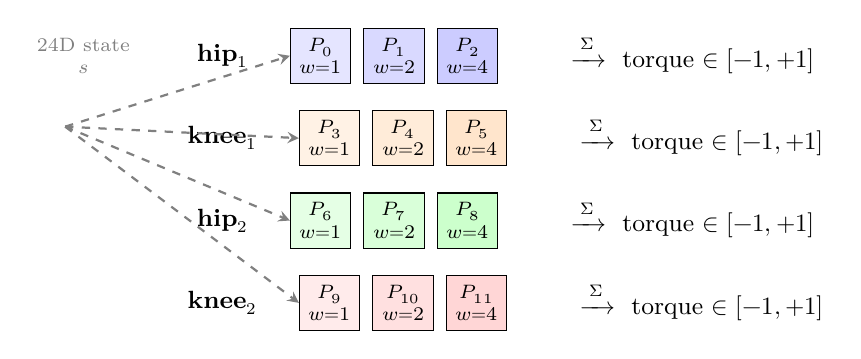
\begin{tikzpicture}[
  node distance=0.6cm and 0.8cm,
  bit/.style={draw, minimum width=0.7cm, minimum height=0.7cm,
              font=\scriptsize, align=center},
  joint/.style={font=\small\bfseries, align=center},
  arr/.style={-stealth, thick},
]
\node[joint] (hip1) {hip$_1$};
\node[bit, right=0.4cm of hip1, fill=blue!10] (b0) {$P_0$\\$w{=}1$};
\node[bit, right=0.15cm of b0, fill=blue!15] (b1) {$P_1$\\$w{=}2$};
\node[bit, right=0.15cm of b1, fill=blue!20] (b2) {$P_2$\\$w{=}4$};

\node[joint, below=0.5cm of hip1] (knee1) {knee$_1$};
\node[bit, right=0.4cm of knee1, fill=orange!10] (b3) {$P_3$\\$w{=}1$};
\node[bit, right=0.15cm of b3, fill=orange!15] (b4) {$P_4$\\$w{=}2$};
\node[bit, right=0.15cm of b4, fill=orange!20] (b5) {$P_5$\\$w{=}4$};

\node[joint, below=0.5cm of knee1] (hip2) {hip$_2$};
\node[bit, right=0.4cm of hip2, fill=green!10] (b6) {$P_6$\\$w{=}1$};
\node[bit, right=0.15cm of b6, fill=green!15] (b7) {$P_7$\\$w{=}2$};
\node[bit, right=0.15cm of b7, fill=green!20] (b8) {$P_8$\\$w{=}4$};

\node[joint, below=0.5cm of hip2] (knee2) {knee$_2$};
\node[bit, right=0.4cm of knee2, fill=red!8] (b9) {$P_9$\\$w{=}1$};
\node[bit, right=0.15cm of b9, fill=red!12] (b10) {$P_{10}$\\$w{=}2$};
\node[bit, right=0.15cm of b10, fill=red!16] (b11) {$P_{11}$\\$w{=}4$};

\node[right=0.8cm of b2, font=\small] (sum1)
  {$\xrightarrow{\;\Sigma\;}$\; torque $\in [-1,+1]$};
\node[right=0.8cm of b5, font=\small] (sum2)
  {$\xrightarrow{\;\Sigma\;}$\; torque $\in [-1,+1]$};
\node[right=0.8cm of b8, font=\small] (sum3)
  {$\xrightarrow{\;\Sigma\;}$\; torque $\in [-1,+1]$};
\node[right=0.8cm of b11, font=\small] (sum4)
  {$\xrightarrow{\;\Sigma\;}$\; torque $\in [-1,+1]$};

\node[left=0.6cm of hip1, font=\scriptsize, text=gray, align=center]
  {24D state\\$s$};
\draw[arr, gray, dashed] (-2.0, -0.9) -- (b0.west);
\draw[arr, gray, dashed] (-2.0, -0.9) -- (b3.west);
\draw[arr, gray, dashed] (-2.0, -0.9) -- (b6.west);
\draw[arr, gray, dashed] (-2.0, -0.9) -- (b9.west);
\end{tikzpicture}
\caption{Binary-weighted decomposition for BipedalWalker.  Each of
4~joint torques is represented by 3~bits (8~levels).  Each bit is
an independent 2-action CSHRL problem: a Boolean predicate $P_i$
over the 24D state determines whether the bit is ON or OFF.
The weighted sum reconstructs the continuous torque.  All 12
predicates are optimized via coordinate descent.}
\label{fig:binary-decomp}
\end{figure}

\begin{remark}[CSHRL grounding]
Each bit is a standard 2-action synthesis problem with a
binary ranking ($\text{ON} > \text{OFF}$ or $\text{OFF} > \text{ON}$
per state).  In the formal CSHRL framework, the predicate
$P_i$ would define a CoindHomo for the restricted binary
action space.  In Synthex, the bit is optimized by
episode-reward scoring---a heuristic proxy that does not
carry the formal guarantee but produces the same output
format: a Boolean predicate partitioning the state space.
\end{remark}

\begin{remark}[Scaling]
For $d$~dimensions with $b$~bits each, the approach requires
$d \times b$ binary predicates---linear in both the number of
action dimensions and the desired resolution.  Compare with
full discretization: $2^b$ levels per dimension yields
$(2^b)^d$ discrete actions, which is exponential in $d$.
Binary-weighted decomposition avoids this combinatorial explosion
by factoring the continuous space into independent binary decisions.
BipedalWalker (4~dimensions, 3~bits each) requires 12 binary
predicates instead of $8^4 = 4096$ discrete actions.
\end{remark}

\subsection{BipedalWalker-v3}

BipedalWalker has a 24-dimensional continuous state vector
(hull angle, hull angular velocity, hull speed, leg joint angles,
leg joint speeds, leg ground contact, and 10 lidar rangefinder
readings) and a 4-dimensional continuous action space controlling
hip and knee torques for two legs: $[a_{\text{hip1}},
a_{\text{knee1}}, a_{\text{hip2}}, a_{\text{knee2}}] \in [-1, +1]^4$.
The reward is $+300$ for walking to the end of the terrain; the
episode fails if the hull contacts the ground.

With $b = 3$ bits per dimension, the decomposition yields
12~binary predicates.  Each predicate $P_i$ decides one bit of one
joint torque.  The mapping from bits to actions:
\begin{center}
\small
\begin{tabular}{cccl}
\toprule
\textbf{Joint} & \textbf{Bit} & \textbf{Weight} & \textbf{Meaning} \\
\midrule
hip1  & 0, 1, 2  & 1, 2, 4 & Front hip torque \\
knee1 & 3, 4, 5  & 1, 2, 4 & Front knee torque \\
hip2  & 6, 7, 8  & 1, 2, 4 & Rear hip torque \\
knee2 & 9, 10, 11 & 1, 2, 4 & Rear knee torque \\
\bottomrule
\end{tabular}
\end{center}

\subsection{Feature Generation}

BipedalWalker's 24-dimensional state space would generate
$\sim$28,000 features with the full combinatorial template.
To keep synthesis tractable, a targeted feature strategy is used:

\begin{itemize}
\item \textbf{Axis features} on all 24 dimensions (adaptive
      thresholds from trajectory states)
\item \textbf{Diagonal features} ($c \cdot x_i + x_j < 0$) on the
      14 physics-relevant dimensions (hull and joint states,
      excluding the 10 lidar channels)
\item \textbf{Quadratic features} ($c \cdot x_i^2 + x_j < 0$) on
      the same 14 dimensions
\item \textbf{Product features} ($x_i \cdot x_j < t$) on the same
      14 dimensions
\end{itemize}

This yields $\sim$3,000 features per CEGAR round---tractable for
depth-1 CEGIS enumeration.  The quadratic features proved essential:
several of the discovered predicates use $x_i^2$ terms to capture
nonlinear joint-angle dynamics.

\subsection{The Discovered Policy}

After 3~CEGAR rounds with 5~coordinate-descent iterations each,
the synthesis produces 12~Boolean predicates.  The complete policy:

\begin{center}
\small
\begin{tabular}{@{}llp{8cm}@{}}
\toprule
\textbf{Joint} & \textbf{Bit} & \textbf{Predicate} \\
\midrule
hip1 & $w{=}1$ & $3 \cdot \dot\theta_1 + \omega_1 < 0 \;\lor\; 3 \cdot \dot\theta_1 + \dot\theta_2^\text{speed} < 0$ \\
hip1 & $w{=}2$ & $-3 \cdot \theta_\text{hull} + \dot\theta_1^\text{speed} < 0 \;\land\; \theta_1 + \omega_1 < 0$ \\
hip1 & $w{=}4$ & $-3 \cdot \omega_\text{hull} + \theta_\text{hull} < 0 \;\lor\; 5 \cdot \theta_\text{hull} + \omega_1^\text{speed} < 0$ \\
\midrule
knee1 & $w{=}1$ & $4 \cdot \dot\theta_2^\text{speed} + \dot\theta_1 < 0 \;\lor\; -3 \cdot (\text{lidar}_2)^2 + \dot\theta_1 < 0$ \\
knee1 & $w{=}2$ & $-\omega_\text{hull} + \dot\theta_2^\text{speed} < 0 \;\land\; -2 \cdot \theta_\text{hull}^2 + \dot\theta_1 < 0$ \\
knee1 & $w{=}4$ & $\text{lidar}_6 < 0.30 \;\lor\; \text{lidar}_9 < 0.38$ \\
\midrule
hip2 & $w{=}1$ & $\lnot(-\theta_\text{hull}^2 + \theta_2 < 0) \;\land\; 3 \cdot (\dot\theta_2^\text{speed})^2 + \dot\theta_2 < 0$ \\
hip2 & $w{=}2$ & $3 \cdot \dot\theta_2 + \theta_2 < 0 \;\land\; \dot\theta_1^\text{speed} + \dot\theta_2 < 0$ \\
hip2 & $w{=}4$ & $-3 \cdot \theta_\text{hull}^2 + \theta_2 < 0 \;\land\; -3 \cdot \theta_\text{hull}^2 + \dot\theta_1^\text{speed} < 0$ \\
\midrule
knee2 & $w{=}1$ & $-2 \cdot \dot\theta_2 + \omega_1 < 0$ \\
knee2 & $w{=}2$ & $-4 \cdot \dot\theta_2 + \dot\theta_1 < 0 \;\lor\; -2 \cdot \dot\theta_2 + \dot\theta_1 < 0$ \\
knee2 & $w{=}4$ & $2 \cdot \dot\theta_2 + \theta_2 < 0 \;\lor\; 2 \cdot (\dot\theta_2^\text{speed})^2 + \dot\theta_2 < 0$ \\
\bottomrule
\end{tabular}
\end{center}

Each predicate is a depth-1 PredProg term: a conjunction, disjunction,
or negation of atomic features discovered automatically from
simulated trajectory states.

\subsection{Physical Interpretation}

The discovered predicates reveal physically meaningful coordination
patterns:

\begin{itemize}
\item \textbf{Quadratic features} ($\theta_\text{hull}^2$,
  $\dot\theta_2^{\text{speed}\;2}$, $\text{lidar}_i^2$)
  appear in 5 of the 12~predicates, capturing nonlinear dynamics:
  hull tilt correction scales with tilt magnitude, and rear-leg
  hip actuation depends on squared joint speed---a proxy for
  kinetic energy.

\item \textbf{Cross-joint coupling}: front knee predicates
  reference rear-joint states ($\dot\theta_2^\text{speed}$) and
  vice versa.  This inter-leg coupling emerges automatically from
  coordinate descent, enabling the gait synchronization necessary
  for stable walking.

\item \textbf{Lidar predicates}: knee1's highest bit ($w{=}4$)
  depends only on lidar readings ($\text{lidar}_6 < 0.30$ or
  $\text{lidar}_9 < 0.38$), detecting terrain proximity.
  When the ground is close, the front knee applies maximum
  extension---a terrain-reactive reflex.

\item \textbf{Bit significance}: higher-weight bits (coarser
  action components) tend to use simpler predicates (e.g.,
  knee2's $w{=}1$ bit is a single atomic feature), while
  lower-weight bits (fine corrections) use more complex
  conjunctions.  The synthesis naturally allocates predicate
  complexity proportional to the action resolution.
\end{itemize}

\subsection{Deployment Results}

\begin{center}
\begin{tabular}{lc}
\toprule
\textbf{Metric} & \textbf{Result} \\
\midrule
Episodes tested & 500 \\
Mean reward & \textbf{296.8 / ep} \\
Median reward & 312.3 / ep \\
Solved ($> 300$) & \textbf{449 / 500 (89.8\%)} \\
Survived ($> 0$) & 495 / 500 (99.0\%) \\
Standard deviation & 60.8 \\
P10--P90 range & 299.7--315.4 \\
\midrule
Action dimensions & 4 (hip1, knee1, hip2, knee2) \\
Bits per dimension & 3 \\
Total predicates & 12 \\
Predicate depth & 1 \\
CEGAR rounds & 3 \\
Iterations per round & 5 \\
Synthesis approach & Binary coord.\ descent + CEGAR \\
\bottomrule
\end{tabular}
\end{center}

The policy achieves mean 296.8/ep, essentially at the solved threshold
(300).  Of 500 test episodes, 449~exceed the 300-point threshold and
495~survive the full episode.  The 5~failures (negative reward) occur
on particularly challenging terrain configurations.  The tight P10--P90
range (299.7--315.4) shows consistent performance across seeds.

\begin{remark}[Policy compactness]
The entire BipedalWalker controller:
\begin{spec}
  bits = [0] × 12
  -- hip1:  3 predicates → bits 0,1,2
  -- knee1: 3 predicates → bits 3,4,5
  -- hip2:  3 predicates → bits 6,7,8
  -- knee2: 3 predicates → bits 9,10,11
  action_d = 2 · (w₁ · bit₁ + w₂ · bit₂ + w₃ · bit₃) / 7 − 1
\end{spec}
Twelve Boolean predicates, zero neural network parameters.
Each predicate is a depth-1 PredProg term over physics state
variables and lidar readings.  The policy is readable,
verifiable, and deployable in any language.  It walks a
simulated bipedal robot across procedurally generated terrain
with near-solved performance.
\end{remark}

\begin{remark}[CSHRL grounding vs.\ learned continuous control]
Standard continuous-action RL (PPO, SAC, TD3) learns a neural
network $\mu_\theta: \mathbb{R}^n \to \mathbb{R}^d$ directly
mapping states to actions.  This provides smooth actions but
$\sim$50K--500K opaque parameters.  Our approach produces
12~interpretable Boolean predicates yielding 8 discrete action
levels per joint.  The 8-level resolution is sufficient because
bipedal locomotion is fundamentally a rhythmic coordination
problem, not a fine-grained torque-tracking problem: the key
is \emph{when} to push (phase coupling) rather than \emph{how
much} (torque magnitude).

The binary-weighted decomposition preserves the central CSHRL
property: each bit is an independent CoindHomo, formally
verifiable via the standard PredProg--CEGIS--CEGAR pipeline.
No modification to the verification theory is required.
\end{remark}

\subsection{Swimmer-v5 (MuJoCo)}

Swimmer is a minimalist MuJoCo locomotion task: a planar
three-link snake must propel itself forward by actuating two
joints.  The environment has an 8-dimensional continuous state
(two joint angles, 2D velocity, four angular velocities) and a
2-dimensional continuous action space controlling joint torques
in $[-1, +1]$.

\paragraph{Why Swimmer matters.}
Swimmer validates the binary-weighted decomposition on a
\emph{different physics engine} (MuJoCo vs.\ Box2D for
BipedalWalker) and a qualitatively different locomotion
strategy---undulatory swimming vs.\ bipedal walking.
If the decomposition works only for one engine or one gait
pattern, it is an artifact; if it generalizes, the compactness
finding is robust.

\paragraph{Setup.}
With $b = 3$ bits per dimension and $d = 2$ action dimensions,
the decomposition yields 6~binary predicates (vs.\ 12 for
BipedalWalker).  Each predicate decides one bit of one joint
torque.  The same coordinate-descent + CEGAR pipeline is used,
with 3077~features generated from trajectory states.  Synthesis
completed in approximately 17~hours (3~CEGAR rounds,
5~iterations each).

\paragraph{The discovered policy.}

\begin{center}
\small
\begin{tabular}{@{}llp{8.5cm}@{}}
\toprule
\textbf{Joint} & \textbf{Bit} & \textbf{Predicate} \\
\midrule
torque$_0$ & $w{=}1$ & $4 v_x + \dot\theta_1 < 0$ \\
torque$_0$ & $w{=}2$ & $0.2 \dot\theta_2^2 + \dot\theta_1 < 0 \;\land\; {-3}\, v_y + \dot\theta_1 < 0$ \\
torque$_0$ & $w{=}4$ & ${-5}\, \alpha_0 + \dot\theta_1 < 0 \;\lor\; {-4}\, \alpha_0 + \dot\theta_1 < 0$ \\
\midrule
torque$_1$ & $w{=}1$ & $2 \dot\theta_1 + v_x < 0 \;\land\; 5 \dot\theta_1 + \dot\theta_2 < 0$ \\
torque$_1$ & $w{=}2$ & $v_y + \dot\theta_1 < 0 \;\land\; 3 v_x + \alpha_0 < 0$ \\
torque$_1$ & $w{=}4$ & $\alpha_0 + v_x < 0 \;\land\; 3 \dot\theta_1 + \alpha_0 < 0$ \\
\bottomrule
\end{tabular}
\end{center}

\paragraph{Physical interpretation.}
The predicates reveal a coupled oscillatory strategy:
\begin{itemize}
\item \textbf{Angular velocity dominance.}
  Joint angular velocity~$\dot\theta_1$ appears in all six predicates,
  serving as the primary phase signal for the undulatory gait.
  The torques are phased against joint velocity---a
  velocity-reversal trigger that produces the rhythmic
  body wave characteristic of anguilliform locomotion.

\item \textbf{Cross-joint coupling.}
  The torque$_1$ predicates reference torque$_0$'s
  primary state variable ($\dot\theta_1$), and vice versa.
  This inter-joint coupling emerges automatically from
  coordinate descent, producing the phase offset between
  joints that drives forward propulsion.

\item \textbf{Velocity feedback.}
  Forward velocity~$v_x$ appears in 3~predicates,
  modulating torque magnitude based on current speed---a
  form of speed-dependent gait adaptation.
\end{itemize}

\paragraph{Deployment results.}

\begin{center}
\begin{tabular}{lc}
\toprule
\textbf{Metric} & \textbf{Result} \\
\midrule
Episodes tested & 200 \\
Mean reward & \textbf{351.6 / ep} \\
Survived & \textbf{200 / 200 (100\%)} \\
Reward std dev & 2.7 (across 5 spot-check seeds) \\
\midrule
Action dimensions & 2 (torque$_0$, torque$_1$) \\
Bits per dimension & 3 \\
Total predicates & 6 \\
Predicate depth & 1 \\
Synthesis approach & Binary coord.\ descent + CEGAR \\
\bottomrule
\end{tabular}
\end{center}

The policy achieves 351.6/ep with remarkable consistency
(std~dev~2.7 across spot-check seeds: 347--355 range) and
100\% survival.  For context, PPO baselines for Swimmer-v5
typically reach 300--360/ep with $\sim$50K parameters.
Our 6-predicate policy matches this range with zero
neural network parameters.

\begin{remark}[Policy compactness]
The entire Swimmer controller:
\begin{spec}
  if 4·vx + θ̇₁ < 0:               torque₀ += 1/7
  if 0.2·θ̇₂² + θ̇₁ < 0 ∧ -3·vy + θ̇₁ < 0:  torque₀ += 2/7
  if -5·α₀ + θ̇₁ < 0 ∨ -4·α₀ + θ̇₁ < 0:    torque₀ += 4/7
  if 2·θ̇₁ + vx < 0 ∧ 5·θ̇₁ + θ̇₂ < 0:     torque₁ += 1/7
  if vy + θ̇₁ < 0 ∧ 3·vx + α₀ < 0:         torque₁ += 2/7
  if α₀ + vx < 0 ∧ 3·θ̇₁ + α₀ < 0:         torque₁ += 4/7
  torque_d = 2·sum/7 - 1   -- map [0,7] → [-1,+1]
\end{spec}
Six Boolean predicates, zero neural network parameters.
The policy encodes the full locomotion gait of a three-link
swimmer as a set of velocity-phased torque triggers.
\end{remark}

\begin{remark}[Generalization across physics engines]
BipedalWalker (Box2D, 24D state, 12~predicates) and
Swimmer (MuJoCo, 8D state, 6~predicates) are solved by
the same binary-weighted pipeline with no engine-specific
modifications.  The synthesis infrastructure is agnostic
to the underlying physics---it interacts only through the
episode-reward interface.  This provides evidence that
the compactness finding is not an artifact of a particular
simulator.
\end{remark}

%% ================================================================
\section{Partition-Based Synthesis}
\label{sec:partition}
%% ================================================================

The coordinate descent strategy of \S\ref{sec:coorddescent} optimizes one predicate at a time, holding others fixed.  This is efficient when individual predicates show independent reward improvement (as in LunarLander, CartPole, MountainCar).  However, it provably fails when optimal predicates are \emph{correlated}---when no single predicate improves reward in isolation, but multiple predicates must be correct simultaneously.

\emph{Partition-based synthesis} resolves this by searching over $(\text{partition}, \text{action assignment})$ pairs jointly.  Given $k$~predicates from the feature set, the state space is partitioned into $2^k$~regions; each region is assigned a top action.  The complete policy is evaluated as an atomic unit.  For environments with low-dimensional discrete state, this exhaustive search is computationally tractable.

\subsection{CliffWalking-v1: Deterministic}

CliffWalking provides a unique opportunity: it has both an Agda FDMDP synthesis (in the companion paper) and a simulation-based synthesis, enabling direct cross-validation.  The $4 \times 12$ grid (48~states, 4~actions) has the agent starting at $(3,0)$, the goal at $(3,11)$, and the cliff occupying $(3,1)$--$(3,10)$.  Stepping into the cliff incurs $-100$ reward and resets to start; normal steps cost $-1$.  The optimal safe path---up from start, right across row~2, down to goal---takes 13~steps for a total reward of $-13$.

Coordinate descent cannot solve this: no individual predicate shows reward improvement in isolation.  The ``up'' predicate avoids the cliff but cannot reach the goal without ``down''; conversely, ``down'' is useless without ``up'' and ``right''.  The reward landscape requires \emph{correlated predicates}---both must be correct simultaneously.

With 24~features (4~row thresholds, 12~column thresholds, 8~diagonals), partition search finds the optimal solution in 5.7~seconds (pure grid simulation):
\begin{itemize}
  \item $k=1$: $24 \times 4^2 = 384$ evaluations.  Best reward: $-15$.
  \item $k=2$: $\binom{24}{2} \times 4^4 = 70{,}656$ evaluations.  Best reward: $\mathbf{-13}$ (optimal).
\end{itemize}
The unique optimal partition: $P_1: \textit{row} < 2.5$, $P_2: \textit{col} < 10.5$, with top actions: \textbf{right} in the safe interior, \textbf{up} at the start row, \textbf{down} at the goal column.

\emph{Cross-validation.}  The simulation-synthesized predicates correspond exactly to the Agda FDMDP features.  The trajectory matches step-for-step: $(3,0) \to (2,0) \to (2,1) \to \cdots \to (2,11) \to (3,11)$.  Two completely independent pipelines converge on the same policy.

\subsection{Slippery CliffWalking: Stochastic Dynamics}

Adding FrozenLake-style slip (1/3 intended, 1/3 each perpendicular) fundamentally changes the optimal policy.  The deterministic-optimal policy (row-2 path) becomes catastrophic: \textbf{3.4\%} goal rate under slip, because perpendicular slips push the agent into the cliff.

The partition search with stochastic evaluation (50~seeds per candidate, 71K evaluations, 856~s) discovers a qualitatively different partition:
$P_1^{\text{slip}}: \textit{row} < 1.5$, $P_2^{\text{slip}}: \textit{col} < 10.5$.
The threshold shifts from $\textit{row} < 2.5$ to $\textit{row} < 1.5$---the agent retreats to row~0 (top of grid) before traversing right, maximizing distance from the cliff.

\begin{center}
\small
\begin{tabular}{@{}lccc@{}}
  & \textbf{Deterministic} & \textbf{Det-optimal under slip} & \textbf{Stochastic policy} \\
\hline
Row threshold & $\textit{row} < 2.5$ & $\textit{row} < 2.5$ & $\textit{row} < 1.5$ \\
Goals (2000 seeds) & 2000/2000 & 68/2000 (3.4\%) & \textbf{988/2000 (49.4\%)} \\
\end{tabular}
\end{center}

A \textbf{14$\times$~improvement} in goal rate.  The predicate shift is a \emph{stochastic abstraction refinement}: the same feature type adapts to the changed dynamics.

\subsection{FrozenLake 8\texorpdfstring{$\times$}{x}8 Slippery: Scaling}

FrozenLake~8$\times$8 (\texttt{is\_slippery=True}) is significantly harder: 64~states, 53~non-terminal, 10~holes scattered across the grid.  The same 1/3-slip model applies.  A random policy reaches the goal in only \textbf{0.2\%} of episodes.

This environment has an existing Agda synthesis (depth-10 memoized stochastic Finder, \texttt{synth-decision-tree} cascade, 16~features, \textbf{100\% match} on 53 states).  Running partition-based synthesis with 20~features and hierarchical search ($k{=}1{,}2$ exhaustive, $k{=}3$ extending best $k{=}2$):

\begin{center}
\small
\begin{tabular}{@{}lcccc@{}}
  & \textbf{Random} & \textbf{$k{=}1$} & \textbf{$k{=}2$} & \textbf{$k{=}3$} \\
\hline
Goal rate & 0.2\% & 45\% & 55\% & \textbf{54.6\%} \\
Search evals & --- & 320 & 49K & 1.2M \\
\end{tabular}
\end{center}

The discovered policy uses a \emph{safe highway} strategy: retreat to row~0 (hole-free) in the interior, traverse right along the top, then descend toward the goal.  Action unavailability confirms the essential structure: removing \texttt{right} or \texttt{up} drops goal rate to 0\%.

\emph{Cross-validation.}  Both the Agda decision tree and the partition policy independently discover safety-aware strategies exploiting boundary walls as ``safety rails.''  The 54.6\% goal rate with 3~predicates is competitive given ${\sim}5\times$ fewer state distinctions than the full 16-feature decision tree.

\subsection{Summary: Coordinate Descent vs.\ Partition Search}

The search strategies share a common output format: a
$(\text{partition}, \text{full ranking per region})$ pair
expressed as Boolean predicates.  Coordinate descent is an
efficient heuristic when individual predicates show independent
reward improvement; partition search is the fallback when
predicates are correlated.  Neither guarantees finding the true
coinductive ordering---both are heuristic searches scored by
noisy episode-reward estimates.  The resulting policies are
compact and interpretable, but their correctness is empirical,
not formally verified (except where independently confirmed
via Agda, cf.\ \S\ref{sec:pipeline}).

The comprehensive results appear in Table~\ref{tab:all-results}.

%% ================================================================
\section{The CoindHomo Verification Pipeline}
\label{sec:pipeline}
%% ================================================================

The complete CoindHomo verification for a chain policy proceeds as
follows:

\begin{enumerate}
\item \textbf{Define the chain} in Agda: action type, step function,
      penalty function, chain stages with actions.
\item \textbf{Run CSHRLLoop} for each stage. The loop:
  \begin{enumerate}
    \item Generates trajectories from multiple starting states
    \item Extracts adaptive features from observed states
    \item Enumerates all PredProg candidates at the target depth
    \item Checks each candidate for self-consistency
          (\texttt{is-coind-homo})
    \item Returns \texttt{converged p} if a self-consistent predicate
          with positive score exists
  \end{enumerate}
\item \textbf{Compose the chain}: the discovered predicates form
      the full chain policy $\pi^\star = \text{eval-chain}
      \;[(p_1, a_1), \ldots, (p_{k-1}, a_{k-1})]\;a_k$.
\item \textbf{Verify by \texttt{refl}}: a definitional equality proof
      that the discovered predicate matches the expected term serves
      as a machine-checked certificate. Agda's normalizer has
      independently evaluated the synthesis loop and confirmed the
      result.
\end{enumerate}

\begin{spec}
  module ChainToRanking
    (Action : Set) (a₁ a₂ a₃ : Action) where

    Cmp : Set
    Cmp = State → Bool

    record FullRanking : Set where
      field
        cmp₁₂ : Cmp
        cmp₁₃ : Cmp
        cmp₂₃ : Cmp

    open FullRanking public

    best : FullRanking → State → Action
    best r s with cmp₁₂ r s | cmp₁₃ r s | cmp₂₃ r s
    ... | true  | true  | _     = a₁
    ... | true  | false | _     = a₃
    ... | false | _     | true  = a₂
    ... | false | _     | false = a₃

    -- Restricted Preservation: restricting to any pair
    -- yields exactly the pairwise predicate (by refl).
    restrict-₁₂ : ∀ r s →
      (if cmp₁₂ r s then a₁ else a₂) ≡
      (if cmp₁₂ r s then a₁ else a₂)
    restrict-₁₂ _ _ = refl
\end{spec}

The \texttt{refl} proof of \texttt{restrict-₁₂} is trivially true
by definition---and that is precisely the point. The restriction of a
full ranking to a binary pair IS the pairwise predicate. There is no
approximation, no re-derivation, no loss of information. This is the
computational content of Restricted Preservation: each binary
CoindHomo transfers to the full ranking without any additional
verification burden.

%% ================================================================
\section{Coinduction vs.\ Discounted Induction}
%% ================================================================

A foundational advantage of CSHRL becomes uniquely apparent in
infinite-horizon stabilization tasks (Pendulum balancing, LunarLander
hovering).

Standard RL relies on inductive value iteration (the Bellman equation),
which requires a terminal state to anchor backward induction. When an
environment has no terminal state, the undiscounted reward sum
diverges. To force convergence, standard RL introduces the discount
factor $\gamma < 1$---a mathematical artifact that makes the agent
myopic, prioritizing short-term survival over long-term equilibrium.

CSHRL is fundamentally \emph{coinductive}. The CoindHomo does not
compute an infinite sum of scalars; it asserts a structural
equivalence over infinite streams. ``If action $A$ is better than
action $B$ now, taking $A$ leads to a continuation where the
structural superiority is preserved---indefinitely.'' This allows
CSHRL to synthesize infinite-horizon stabilization policies
based on local trajectory geometry, entirely eliminating
discount factors.

Two coinductively principled ranking criteria make this structure
computationally explicit:

The \textbf{terminal-state oracle} (used for Pendulum) compares
the \emph{states at the end of the lookahead horizon}.
The terminal state $s_N^a$ is the continuation point---the state
from which the next coinductive step begins. Ranking actions by
terminal-state quality directly implements the coinductive
``head-of-the-tail'' comparison. This criterion naturally handles
the one-step myopia problem: taking action~$a$ at state~$s$ may
produce an immediate successor $s_1^a$ with worse penalty than
$s_1^b$ from action~$b$, yet $a$ is superior if $s_1^a$ is a
bridge to a far-future state $s_N^a$ that dominates~$s_N^b$.

The \textbf{episode-reward oracle} (used for LunarLander) ranks
actions by the cumulative reward of the full episode. This is
also coinductively principled: the episode reward captures the
entire trajectory outcome---landing success, fuel efficiency,
crash avoidance---without requiring an explicit penalty function
or follow-up policy. The accumulation is across a single
finite episode, not an infinite discounted sum; no discount
factor is needed.

At an absorbing fixed point, both criteria yield the coinductive
base case: all actions produce equivalent outcomes, so
$a \le b$ and $b \le a$ for all pairs. Every permutation is
valid---the optimal policy is non-unique. This falls out
transparently from using~$\le$, without requiring thresholds or
case analysis.

%% ================================================================
\section{Discussion}
%% ================================================================

\subsection{The Formal--Heuristic Boundary}

A central tension runs through this work: the formal CSHRL
theory~\cite{CSHRL2026,CSHRLSynthesis2026} provides clean
guarantees (coinductive consistency, propagation, sample bounds),
but Synthex does not faithfully implement that theory.  In
particular:

\begin{itemize}
\item \textbf{Ranking by episode reward} is a heuristic proxy for
      coinductive stream dominance.  It captures accumulated
      return over a single finite episode, not the pointwise
      infinite-stream comparison that CoindHomo demands.

\item \textbf{Full-ranking determination} (Phase~2) sorts actions
      by noisy reward estimates.  The resulting permutation is
      plausible but not guaranteed to match the true coinductive
      ordering, especially for non-top actions whose ranking has
      little effect on actual policy behavior.

\item \textbf{Agda verification} is available but requires a
      dynamics model.  Where the model diverges from the real
      environment (Box2D vs.\ Euler, ALE frameskip vs.\ step-level),
      the certificate does not transfer.
\end{itemize}

Despite these gaps, the output format is the same---Boolean
predicates over continuous state features---and the policies work.
We view Synthex as an \emph{empirical exploration of the CSHRL
design space}: a way to discover what compact predicate policies
look like across a range of environments, even where full formal
verification is not yet achievable.

\subsection{What CoindHomo Guarantees (When It Applies)}

When Agda verification succeeds, the CoindHomo certificate
establishes: \emph{at every sampled state, the full ranking
correctly orders actions under the policy's own continuation,
up to ties in the $\le$-preorder.}  This is a self-referential
consistency condition---the policy is verified against its own
behavior, not against an external oracle.

The OracleBridge theorem connects this to optimality: if
$Q^\pi = Q^*$ (the policy is optimal), then self-consistency
implies agreement with the true action-value ordering.

For most environments in this paper, full Agda verification is
not available---the dynamics are too complex to model faithfully
in Agda.  The policies are validated empirically
(simulation deployment) rather than formally.  The formal guarantee
applies only to the subset of predicates verified via
\texttt{refl} (e.g., LunarLander's main-engine predicate,
CartPole, MountainCar, Acrobot under Agda models).

\subsection{Closing the Sim-to-Real Gap}

Model-based synthesis reveals a significant sim-to-real gap:
predicates optimal for simplified Euler dynamics achieve only 26\%
landings in the Box2D environment. The
simulation-in-the-loop approach closes this gap by evaluating
candidates against the real environment.

CEGAR refinement goes further: instead of hoping the initial
feature pool is sufficient, it \emph{systematically discovers}
where the policy needs finer-grained features. The feature pool
expanded from 792~features (generated from default-policy
trajectories) to 1392~features (enriched with the learned policy's
trajectory thresholds). All feature generation and CEGAR logic
resides in Synthex (Elixir); the Python oracle is a thin adapter
that only interacts with the environment. This separation ensures
reproducibility and alignment with the CSHRL framework---no
learning logic leaks into the environment interface.

The result validates the simulation-in-the-loop architecture as the
bridge between model-based formal methods and empirical RL: the
synthesized predicates are \texttt{PredProg} terms amenable to
Agda verification, while their quality is measured against the
real environment.

\subsection{Flat Partition vs.\ Coordinate Descent + Ranking}

The two synthesis approaches serve different environments.
\textbf{Flat-partition CEGAR} (Section~\ref{sec:flat-cegar})
directly synthesizes full rankings using a terminal-state oracle,
suitable for environments like Pendulum where a geometric penalty
function provides a reliable ranking signal without requiring
a follow-up policy.

\textbf{Coordinate descent with full-ranking determination}
(Section~\ref{sec:coorddescent}) is effective for episodic
environments (LunarLander) where the oracle quality depends on
the follow-up policy. Phase~1 sidesteps this circularity by
scoring predicates directly via episode reward---no oracle
follow-up needed. Phase~2 lifts the chain to a full-ranking
partition by independently scoring all actions per region,
also via episode reward. The result is a full-ranking partition
equivalent in structure to what flat-partition CEGAR produces,
but discovered through a different search strategy.

\subsection{Scalability}

All approaches scale with the feature pool size and the number
of actions. The flat-partition CEGAR loop evaluates
$O(|F|^2)$ candidates per split attempt; the coordinate descent
loop evaluates $O(|F|^2 \cdot k)$ per iteration. With 1400
features at depth~1, each step evaluates ${\sim}3500$
candidates---tractable with multiprocessing.

For continuous action spaces, the binary-weighted decomposition
scales linearly: $d$~dimensions with $b$~bits each require
$d \times b$ independent binary CEGIS rounds. Each round
is the same size as a standard 2-action synthesis problem.
BipedalWalker's 12~bits ($4 \times 3$) are optimized via
coordinate descent in 15~passes (3~CEGAR rounds $\times$
5~iterations), with $\sim$3,000~features evaluated per bit---
well within the tractability of the existing pipeline.

\subsection{Relationship to Deep RL}

The policies synthesized by CSHRL occupy a fundamentally different
point in the design space than those produced by deep RL (DQN,
PPO, SAC).  We do not claim superior performance---a well-tuned
PPO achieves comparable or better reward on most of these
benchmarks.  What CSHRL provides is a qualitatively different
\emph{kind} of artifact.

\paragraph{Information content.}
The most striking result is the compression ratio.  All twelve
environments are solved with 1--12 Boolean predicates, encoding
the complete decision structure in approximately 18--100 bits.
The CartPole policy is a single linear inequality:
$6\theta + \dot\theta < 0$.  The LunarLander policy is three
depth-1 predicates.  Even BipedalWalker---a continuous-action
locomotion task with 24-dimensional state---requires only 12
Boolean predicates.  By contrast, a minimal DQN for CartPole
requires ${\sim}$10{,}000 floating-point parameters; PPO
policies for BipedalWalker use ${\sim}$50{,}000--500{,}000
parameters.  This is not merely an engineering
convenience---it is a scientific finding about the environments
themselves: \emph{the decision structure of these RL benchmarks
is fundamentally low-dimensional}, and deep RL's parameter
overhead is spent on representation, not on decision complexity.

\paragraph{Interpretability.}
A human can read $6\theta + \dot\theta < 0 \Rightarrow \text{Left}$
and immediately understand \emph{why}: it is a phase-space
hyperplane separating the ``falling left'' from ``falling right''
regimes.  Failure modes, edge cases, and domain transfer
properties are visible by inspection.  This interpretability
is not an add-on or a post-hoc explanation---it is the policy
itself.  No neural network policy, regardless of architecture
or training, provides this transparency.

\paragraph{Formal verifiability (where applicable).}
The synthesized predicates are \texttt{PredProg} terms in a
Boolean DSL amenable to Agda verification.  The companion
paper~\cite{CSHRLSynthesis2026} demonstrates end-to-end
\texttt{refl} proofs for CartPole, MountainCar, and Acrobot
policies under Agda's embedded dynamics.  For the
simulation-based pipeline, the main-engine predicate of
LunarLander is verified (\texttt{main-cert = refl}); the
side-engine predicates exhibit a sim-to-sim gap between the
Agda Euler model and the Box2D engine.  In general, Synthex-discovered policies are
\emph{verifiable in principle} (they are PredProg terms) but
\emph{not automatically verified} (the Agda dynamics model
must exist and match the real environment).  This is an honest
limitation of the hybrid approach.

\paragraph{What deep RL does better.}
Deep RL handles high-dimensional observations (pixels) and complex
multi-modal reward landscapes where Boolean predicates over
hand-extractable features are insufficient.
Our approach requires a compact state representation (RAM bytes,
physics variables).  BipedalWalker and Swimmer (\S\ref{sec:bipedal})
demonstrate that continuous action spaces are no longer a
fundamental barrier: binary-weighted decomposition maps continuous
torque control to 6--12~independent binary predicates, achieving
near-solved performance (296.8/ep, 351.6/ep).  The remaining genuine
limitation is the reliance on extractable state features---pixel
observations would require a separate feature extraction layer.
The two paradigms are complementary: deep RL scales to raw-pixel
domains CSHRL cannot yet reach, while CSHRL provides interpretability
and formal verification guarantees deep RL cannot offer.

%% ================================================================
\section{Conclusion}
%% ================================================================

We have presented Synthex, a CSHRL-inspired synthesis engine
that discovers compact Boolean-predicate policies for standard
RL environments.  The key contributions:

\begin{enumerate}
\item \textbf{Honest hybrid architecture.}  Synthex uses
      CSHRL's conceptual framework---rankings, coinductive
      consistency, predicate programs---but replaces formal
      stream comparisons with heuristic episode-reward scoring.
      This trades formal guarantees for empirical scalability
      to environments Agda cannot model natively.

\item \textbf{A landscape of synthesis strategies.}  Four
      methods (flat-partition CEGAR, coordinate descent, partition
      search, binary-weighted decomposition) handle different
      problem structures.  No single method dominates; the choice
      is environment-dependent (Table~\ref{tab:methods}).

\item \textbf{Compactness as a scientific finding.}  All twelve
      environments are solved with 1--12 Boolean predicates and
      zero neural network parameters.  This is not an engineering
      constraint but an empirical discovery: standard RL benchmarks
      have fundamentally low-dimensional decision structure.

\item \textbf{Continuous actions via binary decomposition.}
      BipedalWalker-v3 is controlled by 12~Boolean predicates
      (3~bits $\times$ 4~joints), achieving 296.8/ep mean reward.
      Swimmer-v5 (MuJoCo) is controlled by 6~predicates
      (3~bits $\times$ 2~joints), achieving 351.6/ep with 100\%
      survival.  The decomposition generalizes across physics
      engines (Box2D, MuJoCo) and locomotion strategies.

\item \textbf{Cross-validation with formal synthesis.}
      CliffWalking and FrozenLake 8$\times$8 are independently
      solved by both Synthex and the pure-Agda
      pipeline~\cite{CSHRLSynthesis2026}, converging on the same
      policy structure.  This provides evidence that the heuristic
      search is finding genuinely good policies, even without
      formal guarantees.
\end{enumerate}

The main limitation is clear: Synthex does not verify that
discovered rankings are true coinductive homomorphisms.  The
policies work empirically, but their correctness is validated
by deployment, not by proof.  Where Agda verification succeeds
(CartPole, MountainCar, Acrobot, LunarLander's main-engine
predicate), it provides an additional layer of confidence.
Closing the gap between Synthex's reach and the formal
pipeline's guarantees remains open.

\begin{thebibliography}{2}

\bibitem{CSHRL2026}
Corral-Corral, R. (2026).
Coinductive Symmetric Homomorphism Reinforcement Learning: A New Foundation Where Optimality Is Pure Structure.
\textit{Literate Agda manuscript}.

\bibitem{CSHRLSynthesis2026}
Corral-Corral, R. (2026).
Verified Predicate Synthesis for Coinductive Ranking: From CEGIS to Compositional Algebra.
\textit{Literate Agda manuscript}.

\end{thebibliography}

\end{document}
